% Fixing: Too many math alphabets used in version normal
\newcommand\hmmax{0}
\newcommand\bmmax{0}
\documentclass[dvipsnames,conference]{IEEEtran}

\usepackage[T1]{fontenc}
\usepackage[scaled=.83]{beramono}

\usepackage[colorinlistoftodos]{todonotes}
\usepackage[inference]{semantic}
\usepackage[switch]{lineno}
\usepackage{halloweenmath}
\usepackage{fontawesome5}
\usepackage{listofitems}
\usepackage{breakcites}
\usepackage{glossaries}
\usepackage{hyperref}
\usepackage{cleveref}
\usepackage{stmaryrd}
\usepackage{marvosym}
\usepackage{listings}
\usepackage{amssymb}
\usepackage{amsmath}
\usepackage{nameref}
\usepackage{amsthm}
\usepackage{xspace}
\usepackage{xfrac}
\usepackage{tikz}
\usepackage{soul}
\usepackage{bm}

\hypersetup{
    colorlinks,
    linkcolor={red!50!black},
    citecolor={blue!50!black},
    urlcolor={blue!80!black}
}
%\renewcommand\UrlFont{\color{blue}\rmfamily}
%\newcommand{\url}[1]{\lstinline{#1}}

\setul{0.95ex}{0.3ex}


\usetikzlibrary{calc,decorations.pathmorphing,shapes,positioning}
\newcounter{sarrow}
\newcommand\xrsquigarrow[1]{%
\stepcounter{sarrow}%
\mathrel{\begin{tikzpicture}[baseline= {( $ (current bounding box.south) + (0,-0.5ex) $ )}]
\node[inner sep=.5ex] (\thesarrow) {$\scriptstyle #1$};
\path[draw,<-,decorate,
  decoration={zigzag,amplitude=0.7pt,segment length=1.2mm,pre=lineto,pre length=4pt}]
    (\thesarrow.south east) -- (\thesarrow.south west);
\end{tikzpicture}}%
}
\makeatletter
\newcommand{\xRightarrow}[2][]{\ext@arrow 0359\Rightarrowfill@{#1}{#2}}
\makeatother

\newcommand{\thmref}[1]{\cref{#1}~(\nameref{#1})}
\newcommand{\Thmref}[1]{\Cref{#1}~(\nameref{#1})}

%%%%
% TODO macros
\newcommand{\MK}[1]{\todo[color=orange!30]{TODO: #1}}
\newcommand{\MKin}[1]{\todo[color=orange!30,inline]{TODO: #1}}
\newcommand{\MP}[1]{\todo[color=blue!30]{TODO: #1}}
\newcommand{\MPin}[1]{\todo[color=blue!30,inline]{TODO: #1}}
\newcommand{\hltt}[1]{\begin{center}\fbox{\color{green}\large{#1}}\end{center}}

% Approx
\newcommand{\pages}[1]{}%\xspace\todo{\textbf{($\sim$#1 pages)}\xspace}}

%%%%
% Colors
\newcommand{\neutcol}[0]{black}
\newcommand{\stlccol}[0]{RoyalBlue}
\newcommand{\irccol}[0]{Apricot}
\newcommand{\ulccol}[0]{RedOrange}
\newcommand{\objcol}[0]{Emerald} %CarnationPink}
\newcommand{\commoncol}[0]{black}

\newcommand{\col}[2]{\ensuremath{{\color{#1}{#2}}}}

\newcommand{\com}[1]{\ensuremath\mathit{\col{\neutcol}{#1}}}
\newcommand{\src}[1]{\ensuremath\mathsf{\col{\stlccol}{#1}}}
\newcommand{\irl}[1]{\ensuremath\mathit{\col{\irccol}{#1}}}
\newcommand{\trg}[1]{\ensuremath\mathbf{\col{\ulccol}{#1}}}
\newcommand{\obj}[1]{\ensuremath\mathtt{\col{\objcol}{#1}}}

%%%%
% Text Decorations
\newcommand\BrText[2]{%
  \par\smallskip
   \noindent\makebox[\textwidth][r]{$\text{\scriptsize #1}\left\{
    \begin{minipage}{\textwidth}
    #2
    \end{minipage}
  \right.\nulldelimiterspace=0pt$}\par\smallskip
}
\newcommand{\mi}[1]{\ensuremath{\mathit{#1}}}
\newcommand{\mr}[1]{\ensuremath{\mathrm{#1}}}
\newcommand{\mt}[1]{\ensuremath{\texttt{#1}}}
\newcommand{\mtt}[1]{\ensuremath{\mathtt{#1}}}
\newcommand{\mf}[1]{\ensuremath{\mathbf{#1}}}
\newcommand{\mk}[1]{\ensuremath{\mathfrak{#1}}}
\newcommand{\mc}[1]{\ensuremath{\mathcal{#1}}}
\newcommand{\ms}[1]{\ensuremath{\mathsf{#1}}}
\newcommand{\mb}[1]{\ensuremath{\mathbb{#1}}}
\newcommand{\msc}[1]{\ensuremath{\mathscr{#1}}}

\newcommand{\bul}[1]{{\setulcolor{RoyalBlue}\ul{#1}}}
\newcommand{\rul}[1]{{\setulcolor{RedOrange}\ul{#1}}}
\newcommand{\iul}[1]{{\setulcolor{Apricot}\ul{#1}}}
\newcommand{\oul}[1]{{\setulcolor{Emerald}\ul{#1}}}
\newcommand{\pul}[1]{{\setulcolor{CarnationPink}\ul{#1}}}

\newcommand{\lock}{\ensuremath\text{\scriptsize\faIcon{lock}}}
\newcommand{\unlock}{\ensuremath\text{\scriptsize\faIcon{lock-open}}}

\newcommand{\tup}[2]{\ensuremath (#1 %
  \readlist\myterms{#2}%
  \foreachitem\x\in\myterms{;\x}%
  )%
}

\newcommand{\isdef}[0]{\ensuremath{\mathrel{\overset{\makebox[0pt]{\mbox{\normalfont\tiny\sffamily def}}}{=}}}}

%%%%
% List of contributions
\newcounter{contrib}
\newcommand{\contribnum}[0]{\stepcounter{contrib}{\arabic{contrib}}.~}
\newcommand{\contribution}[1]{\smallskip\noindent\textbf{{#1.}\xspace}}

%%%%
% A symbol for Coq-verified theorems.
\newcommand{\BareCoqSymbol}{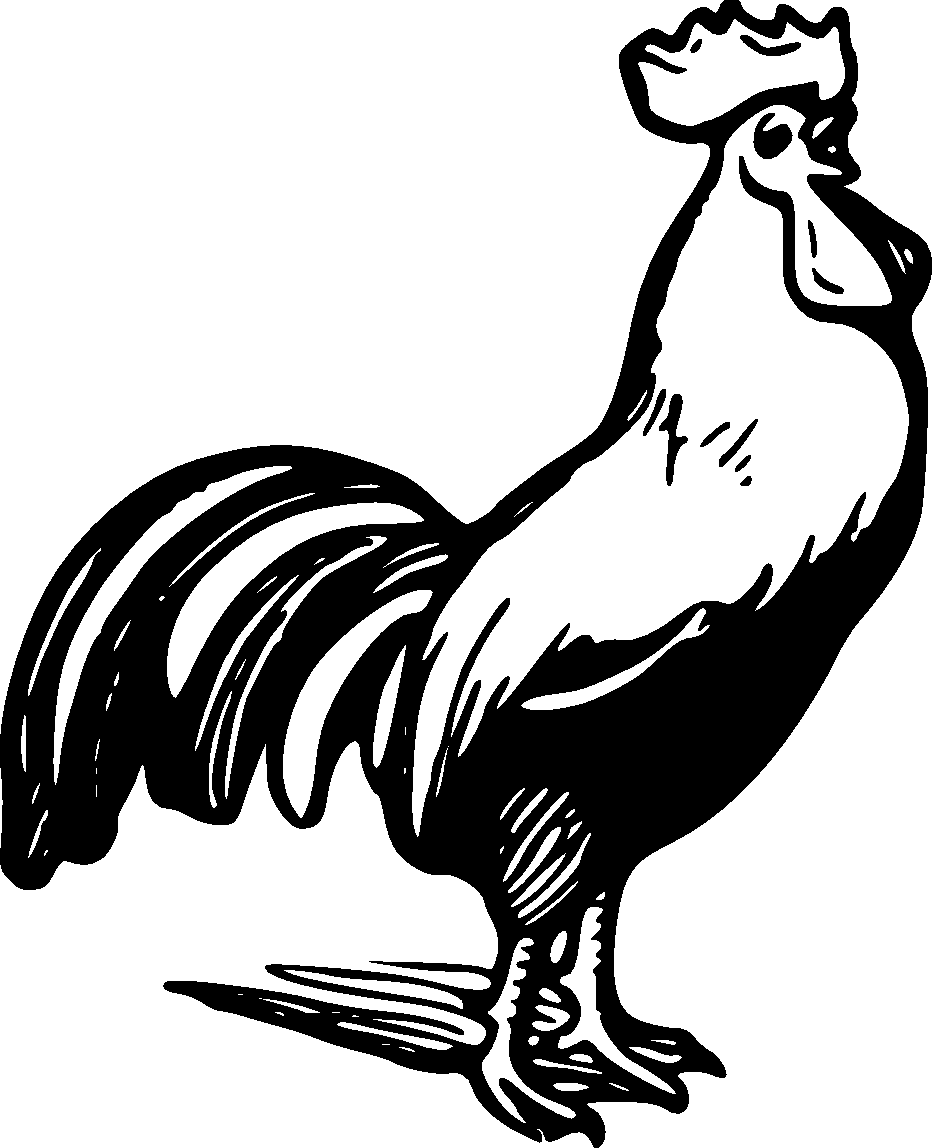
\includegraphics[height=0.9em]{coq.pdf}}
\newcommand{\CoqSymbol}{\raisebox{-.2ex}{\BareCoqSymbol\,}}
\newcommand{\Coqed}{\hfill\CoqSymbol}

\newcommand{\BareInvCoqSymbol}{
\includegraphics[height=0.9em]{inv_coq.png}}
\newcommand{\InvCoqSymbol}{\raisebox{-.2ex}{\BareInvCoqSymbol\,}}

%%%%
% Typerules
\newcommand{\textgraybox}[1]{\boxed{#1}}
\newdimen\zzfontsz
\newcommand{\fontsz}[2]{\zzfontsz=#1%
{\fontsize{\zzfontsz}{1.2\zzfontsz}\selectfont{#2}}}
\newcommand{\mathsz}[2]{\text{\fontsz{#1}{$#2$}}}
\newcommand{\instsymColon}{%
     \raisebox{-0.09ex}{\text{\normalfont{:}}}}
\newcommand{\judgboxfontsize}[1]{%
        \mathsz{11pt}{#1}%
}
\newcommand{\judgbox}[2]{%
      {\raggedright \textgraybox{\ensuremath{\judgboxfontsize{#1}}}\!%
        \fontsz{9pt}{\begin{tabular}[c]{l} #2 \end{tabular}} %
}}
\newcounter{typerule}
\crefname{typerule}{rule}{rules}

\newcommand{\typeruleInt}[5]{%
	\def\thetyperule{#1}%
	\refstepcounter{typerule}%
	\label{tr:#4}%
	%
  \ensuremath{\begin{array}{c}#5 \inference{#2}{#3}\end{array}}
}
\newcommand{\typerule}[4]{%
  \typeruleInt{#1}{#2}{#3}{#4}{\textsf{\scriptsize ({#1})} \\      }
}
\newcommand{\typerulenolabel}[3]{%
	\def\thetyperule{#1}%
	\refstepcounter{typerule}%
  \ensuremath{\begin{array}{c} \inference{#2}{#3}\end{array}}
}
\newcommand{\typerulederiv}[3]{%
  \ensuremath{\begin{array}{c} \inference{#2}{#3} #1\end{array}}
}

%%%%
% Language-specific definitions
% names of properties
\newcommand{\tmssafe}{\ensuremath\operatorname{tms}}
\newcommand{\smssafe}{\ensuremath\operatorname{sms}}
\newcommand{\mssafe}{\ensuremath\operatorname{ms}}
\newcommand{\scctsafe}{\ensuremath\operatorname{scct}}
\newcommand{\msscctsafe}{\ensuremath\operatorname{msscct}}

% Languages
\newcommand{\Ltms}{\ensuremath\src{L_{\tmssafe}}}
\newcommand{\Ltrg}{\ensuremath\trg{L}}
\newcommand{\Lms}{\ensuremath\irl{L_{\mssafe}}}
\newcommand{\Lscct}{\ensuremath\obj{L_{\scctsafe}}}

% Traces
\newcommand{\event}[1][]{a#1}
\newcommand{\absevent}[1][]{\ensuremath\bm{\event[#1]}}
\newcommand{\emptyevent}{\ensuremath\varepsilon}
\newcommand{\trace}[1][]{\ensuremath\overline{a#1}}
\newcommand{\class}[1][]{\ensuremath\mb{C}}
\newcommand{\lift}[1]{\ensuremath\lfloor\xspace{#1}\xspace\rfloor}
\newcommand{\hole}[1]{\ensuremath{\left[#1\right]}}
\newcommand{\ev}[1]{\text{#1}}
\newcommand{\absev}[1]{\ensuremath\bm{#1}}
\newcommand{\abstrace}[1][]{\ensuremath\bm{\trace[]}#1}
\newcommand{\absterm}{\ensuremath\lightning{\kern-5.5pt}\lightning}

% Trace Relations
\newcommand{\traceagree}[4][^*]{\ensuremath{#3}\cong_{#2}#1{#4}}
\newcommand{\tmstraceagree}[3][^*]{\traceagree[#1]{\tmssafe}{#2}{#3}}
\newcommand{\smstraceagree}[3][^*]{\traceagree[#1]{\smssafe}{#2}{#3}}
\newcommand{\mstraceagree}[3][^*]{\traceagree[#1]{\mssafe}{#2}{#3}}
\newcommand{\sccttraceagree}[3][^*]{\traceagree[#1]{\scctsafe}{#2}{#3}}

% Monitors
\newcommand{\monitor}[1][]{\ensuremath T#1}
\newcommand{\tmsmonitor}[1][]{\monitor[_{TMS}{#1}]}
\newcommand{\smsmonitor}[1][]{\monitor[_{SMS}{#1}]}
\newcommand{\scctmonitor}[1][]{\monitor[_{sCCT}{#1}]}
\newcommand{\msmonitor}[1][]{\monitor[_{MS}{#1}]}
\newcommand{\monitorcheck}[4][{\kern-3.5pt}^*]{%
  \vdash\xspace{#2}\xspace \xrsquigarrow{#4}{#1}\xspace{#3}\xspace%
}
\newcommand{\monsafe}[2]{\ensuremath\vdash_{mon}{#1}:{#2}}

\newcommand{\abssecuritytag}[1][]{\ensuremath\bm{\sigma}#1}

\newcommand{\montmssafe}[1]{\monsafe{#1}{\tmssafe}}
\newcommand{\monsmssafe}[1]{\monsafe{#1}{\smssafe}}
\newcommand{\monmssafe}[1]{\monsafe{#1}{\mssafe}}
\newcommand{\monscctsafe}[1]{\monsafe{#1}{\scctsafe}}
\newcommand{\monmsscctsafe}[1]{\monsafe{#1}{\msscctsafe}}

% Languages
\newcommand{\LTMS}{\src{L_{TMS}}}
\newcommand{\LT}{\trg{L}}
\newcommand{\LMS}{\irl{L_{MS}}}
\newcommand{\LCCT}{\obj{L_{sCCT}}}

\newcommand{\bnfdef}{\ensuremath{\mathrel{::=}}}

% Substitution
\newcommand{\subst}[2]{\ensuremath \hole{#1\text{ for }#2}}
\newcommand{\substvar}[1][]{\ensuremath \gamma#1}
\newcommand{\substlist}[1][]{\ensuremath \overline{\gamma#1}}

\newcommand{\partialeval}[2]{\ensuremath \operatorname{\mathtt{mix}}(#1, #2)}

% Predefined Sets
\newcommand{\nat}{\ensuremath\mb{N}}

% Types
\newcommand{\natt}{\ensuremath\mb{N}_t\xspace}
\newcommand{\ptrqual}[1][]{\ensuremath\xspace q#1\xspace}
\newcommand{\fullq}{1\xspace}
\newcommand{\halfq}{\sfrac{1}{2}\xspace}
\newcommand{\ptrn}[1][\ptrqual]{\ensuremath\xspace ref_{#1}\ \natt\xspace}
\newcommand{\wptr}{\ensuremath\ptrn[\halfq]\xspace}
\newcommand{\ptr}{\ensuremath\ptrn[\fullq]\xspace}
\newcommand{\type}[1][]{\ensuremath\tau#1\xspace}
\newcommand{\typenv}[1][]{\ensuremath\Gamma#1\xspace}

% Terms
\newcommand{\wrapkeyword}[2][]{\ensuremath{#1{#2}}}
\newcommand{\expr}[1][]{e#1\xspace}
\newcommand{\ectx}[1][]{K#1\xspace}
\newcommand{\finalexpr}[1][]{f#1\xspace}
\newcommand{\valueexpr}[1][]{v#1\xspace}
\newcommand{\lbinop}[3][]{\ensuremath {#2}{#1{\oplus}}{#3}\xspace}
\newcommand{\lget}[3][]{\ensuremath #2{#1{[}}{#3}{#1{]}}\xspace}
\newcommand{\lset}[4][]{\ensuremath #2{#1{[}}{#3}{#1{]\leftarrow}}#4\xspace}
\newcommand{\lnew}[3][]{\ensuremath \wrapkeyword[#1]{new}\ #2\ {#1{[}}#3{#1{]}}\xspace}
\newcommand{\llet}[4][]{\ensuremath \wrapkeyword[#1]{let}\ #2 {#1{=}} #3\ \wrapkeyword[#1]{in}\ #4\xspace}
\newcommand{\ldelete}[2][]{\ensuremath \wrapkeyword[#1]{delete}\ #2\xspace}
\newcommand{\lreturn}[2][]{\ensuremath \wrapkeyword[#1]{return}\ #2\xspace}
\newcommand{\lcall}[3][]{\ensuremath \wrapkeyword[#1]{call}\ #2\ #3\xspace}
\newcommand{\lifz}[4][]{\ensuremath \wrapkeyword[#1]{ifz}\ #2\ \wrapkeyword[#1]{then}\ #3\ \wrapkeyword[#1]{else}\ #4\xspace}
\newcommand{\labort}[1][]{\ensuremath \wrapkeyword[#1]{abort()}\xspace}
\newcommand{\lispoisoned}[2][]{\ensuremath #2\ \wrapkeyword[#1]{is\ }{#1{\poisoned}}\xspace}
\newcommand{\lpair}[3][]{\ensuremath {#1{\langle}} #2 {#1{;}} #3 {#1{\rangle}} \xspace}
\newcommand{\lproja}[2][]{\ensuremath {#2}{#1{.0}} \xspace}
\newcommand{\lprojb}[2][]{\ensuremath {#2}{#1{.1}} \xspace}
\newcommand{\lhast}[3][]{\ensuremath {#2}\ \wrapkeyword[#1]{has}\ #3 \xspace}
\newcommand{\lwrdoit}[2][]{\ensuremath \wrapkeyword[#1]{wrdoit}\ #2\xspace}
\newcommand{\lrddoit}[3][]{\ensuremath \wrapkeyword[#1]{rddoit}\ #2\ \wrapkeyword[#1]{in}\ #3\xspace}
\newcommand{\function}[1][]{F#1\xspace}
\newcommand{\lfunction}[4][]{\ensuremath\wrapkeyword[#1]{fn}\ {#2}\ {#3}\ {#1{:=}}\ #4\xspace}
\newcommand{\prog}[3][]{\ensuremath\wrapkeyword[#1]{\langle}\ #2; #3\wrapkeyword[#1]{\rangle}\xspace}

% Compiler
\newcommand{\rtp}[2]{\ensuremath\vdash{#1}:{#2}}
\newcommand{\ccbase}[1][]{\ensuremath\gamma{#1}}
\newcommand{\cc}[3][]{\ensuremath{\ccbase[#1]}^{#2}_{#3}\xspace}
\newcommand{\cca}{\ensuremath\cc{\Ltms}{\Ltrg}}
\newcommand{\ccb}{\ensuremath\cc{\Ltrg}{\Lms}}
\newcommand{\ccdce}{\ensuremath\cc[_{\gls{dce}}]{\Lms}{\Lms}}
\newcommand{\cccf}{\ensuremath\cc[_{\gls{cf}}]{\Lms}{\Lms}}
\newcommand{\ccscct}{\ensuremath\cc{\Lms}{\Lscct}}
\newcommand{\ccmsscct}{\ensuremath\cc{\Ltms}{\Lscct}}

% Backtranslation
\newcommand{\backbase}[1][]{\ensuremath\wp#1}
\newcommand{\backt}[3][]{\ensuremath{}^{#2}_{#3}\backbase[#1]}

% Satisfaction
\newcommand{\contextvar}[1][]{C#1}
\newcommand{\progvar}[1][]{p#1}
\newcommand{\wholeprogvar}[1][]{w#1}
\renewcommand{\class}[1][]{\mathbb{C}#1}
\newcommand{\link}[2]{\ensuremath\operatorname{link}\left({#1};{#2}\right)}
\newcommand{\behav}[1]{\ensuremath\operatorname{behav}\left({#1}\right)}
\newcommand{\sat}[2]{\ensuremath\vdash{#1}:{#2}}
\newcommand{\rsat}[2]{\ensuremath\vdash_R{#1}:{#2}}

% State
\newcommand{\securitytag}[1][]{\ensuremath\sigma#1}
\newcommand{\sandboxtag}[1][]{t#1}
\newcommand{\ctx}{\text{ctx}}
\newcommand{\comp}{\text{comp}}
\newcommand{\loc}[1][]{\ensuremath l#1}
\newcommand{\poison}{\ensuremath\rho}
\newcommand{\poisoned}{\ensuremath\text{\Biohazard}}
\newcommand{\poisonless}{\ensuremath\square}
\newcommand{\store}[1][]{\ensuremath\Delta#1}
\newcommand{\storeel}[5]{\ensuremath #1\mapsto\tup{#2}{#3,#4,#5}}
\newcommand{\comm}[1][]{\ensuremath c#1}
\newcommand{\ctxtocomp}{\ensuremath\xspace ? \xspace}
\newcommand{\comptoctx}{\ensuremath\xspace ! \xspace}
\newcommand{\nocomm}{\ensuremath\xspace \varnothing \xspace}
\newcommand{\heap}[1][]{\ensuremath H#1}
\newcommand{\ectxstack}[1][]{\ensuremath\overline{\ectx#1}}
\newcommand{\library}[1][]{\ensuremath\Xi#1}
\newcommand{\commlib}[1][]{\ensuremath\xi#1}
\newcommand{\cfstate}[1][]{\ensuremath\Psi#1}
\newcommand{\memstate}[1][]{\ensuremath\Phi#1}
\newcommand{\statevar}[1][]{\ensuremath\Omega#1}
\newcommand{\rtt}[2]{\ensuremath #1 \triangleright #2}
\newcommand{\growh}[2]{\ensuremath #1 \ll #2}
\newcommand{\seth}[3]{\ensuremath #1(#2 \mapsto #3)}

% Various Judgements
\newcommand{\fresh}[2]{\ensuremath{#1}\vdash{#2}\xspace\operatorname{fresh}\xspace}
\newcommand{\tcheck}[3]{\ensuremath{#1}\vdash{#2}:{#3}\xspace}
\newcommand{\notowned}[1]{\ensuremath\vdash{#1}\xspace\operatorname{not-owned}\xspace}
\newcommand{\typenvsplit}[2]{\ensuremath {#1}\odot{#2}\xspace}
\newcommand{\hastype}[2]{\ensuremath{#1}:{#2}\xspace}
\newcommand{\inttype}[1]{\ensuremath\vdash{#1}\operatorname{int-\type}\xspace}

\newcommand{\thelocmap}{\ensuremath\delta\xspace}
\newcommand{\locmapsto}[2]{\ensuremath\thelocmap({#1})={#2}\xspace}

% Filters
\newcommand{\filter}[4][]{\ensuremath \operatorname{Proj}^{#1}_{#2}\left({#3}, {#4}\right)\xspace}
\newcommand{\msfilterLtms}[2][{\thelocmap}]{\ensuremath\filter[{\Ltms}]{}{#1}{#2}}
\newcommand{\msfilterLms}[2][{\thelocmap}]{\ensuremath\filter[{\Lms}]{}{#1}{#2}}
\newcommand{\msfilterL}[2][{\thelocmap}]{\ensuremath\filter[{\Ltrg}]{}{#1}{#2}}
\newcommand{\scctfilterLms}[2][{\thelocmap}]{\ensuremath\filter[{\Lms}]{}{#1}{#2}}
\newcommand{\scctfilterLscct}[2][{\thelocmap}]{\ensuremath\filter[{\Lscct}]{}{#1}{#2}}

% Steps
\newcommand{\isval}[1]{\ensuremath\vdash{#1}\xspace\operatorname{is-val}\xspace}
\newcommand{\runtimetermvar}[1][]{r#1}
\newcommand{\stepto}[4][{\kern-4.5pt}^*]{\ensuremath{#2}\xrightarrow{#4}{}\xspace{#1}\xspace{#3}\xspace}
\newcommand{\stepton}[4][n]{\ensuremath{#2}\xrightarrow{#4}{}{\kern-3.5pt}^{#1}\xspace{#3}\xspace}

\newcommand{\pstepto}[3]{\ensuremath{#1}\xrightarrow{#3}_p{}\xspace{#2}\xspace}
\newcommand{\estepto}[4][{\kern-4.5pt}^*]{\ensuremath{#2}\xrightarrow{#4}#1_{\operatorname{ectx}}\xspace{#3}\xspace}
\newcommand{\estepton}[4][n]{\ensuremath{#2}\xrightarrow{#4}_{\operatorname{ectx}}{}{\kern-14.5pt}^{#1\ \ \ \;}\xspace{#3}\xspace}
\newcommand{\progstepto}[3]{\ensuremath{#1}\xRightarrow{#3}{#2}}


% allow page breaks inside multiline alignment displays
\allowdisplaybreaks

\Crefname{exampleenv}{Example}{Examples}

\theoremstyle{definition}
\newtheorem{exampleenv}{Example}[section]
\newtheorem{lemma}{Lemma}[section]
\newtheorem{theorem}{Theorem}[section]
\newtheorem{corollary}{Corollary}[section]
\newtheorem{definition}{Definition}[section]

\loadglsentries{acronyms}
\makeglossaries

\AtBeginDocument{%
  \providecommand\BibTeX{{%
    \normalfont B\kern-0.5em{\scshape i\kern-0.25em b}\kern-0.8em\TeX}}}
\makeatletter
\newcommand{\linebreakand}{%
  \end{@IEEEauthorhalign}
  \hfill\mbox{}\par
  \mbox{}\hfill\begin{@IEEEauthorhalign}
}
\makeatother

\renewcommand\thelinenumber{\color{red}\arabic{linenumber}}
\begin{document}
\linenumbers

\title{Secure Composition \\ of Robust and Optimising Compilers}

\author{\vspace*{-2em}\phantom{a}}
% Matthis Kruse\orcidID{0000-0003-4062-9666}
% \and
% Michael Backes
% \and
% Marco Patrignani
% }
% \authorrunning{M. Kruse et al.}

\maketitle

\begin{abstract}
% \MPpost{
%   this abstract fails in setting up the robustness argument.
%   it'll be a good exercise for you to take inspiration from this, but then write something as concise but with a more direct focus on robust properties
% }
% context
To ensure that secure applications do not leak their secrets, they are required to uphold several security properties such as spatial and temporal memory safety, cryptographic constant time, as well as speculative safety.
% need
Existing work shows how to enforce these properties individually, in an architecture-independent way, by using secure compiler passes that each focus on an individual property.
% task
Unfortunately, given two secure compiler passes that each preserve a possibly different security property, it is unclear what kind of security property is preserved by the composition of those secure compiler passes.
%there is no way to tell what kind of security property will the composition of those secure compilers preserve.

% object
This paper is the first to study what security properties are preserved across the composition of different secure compiler passes.
% findings
Starting from a general theory of property composition for security-relevant properties (such as the aforementioned ones), this paper formalises a theory of composition of secure compilers.
Then, it showcases this theory on a secure multi-pass compiler that preserves the aforementioned security-relevant properties.
% conclusion
Crucially, this paper derives the security of the multi-pass compiler from the composition of the security properties preserved by its individual passes, which include security-preserving as well as optimisation passes.
% 
From an engineering perspective, this is the desirable approach to building secure compilers.
\begin{center}\small\it
	{This paper uses syntax highlighting accessible to both colourblind and black \& white readers.
	% ~\cite{patrignani2020use}.
% 	% Specifically, it makes use of a $\src{blue}$, $\src{sans\text{-}serif}$ font for a $\src{source}$,
% 	% a $\trg{red}$, $\trg{bold}$ font for an $\trg{intermediate}$,
% 	% and a $\obj{green}$, $\obj{teletype}$ font for a $\obj{target}$ language.	
	Please print or view in colours.
	}
\end{center}
\end{abstract}

\begin{IEEEkeywords}
  memory-safety, cryptographic constant-time, secure compilation, robustness
\end{IEEEkeywords}

\section{Introduction\pages{4}}\label{sec:introduction}

% \gls*{ms} is a security property that ensures that there are no out-of-bounds accesses as well as no reads or writes to uninitialised memory.
% Programs that do not attain memory safety, can easily have their private data be leaked to attackers or be corrupted~\cite{lemay2021ccc}.
% Because of this, \gls*{ms} is a requirement for programs to attain an even stronger security property, namely \gls*{cct}.
% Programs that attain \gls*{cct} are secure w.r.t. timing attacks, and this is the gold standard for secure applications, including cryptographic ones, since timing attacks can expose secrets via a simple performance analysis~\cite{kocher1996timing}.
% Timing attacks have become more and more relevant recently, especially given the era of cloud-computing~\cite{aviram2010cloudtime,kumar2019cloudsecsurvey}, where programs share the same hardware but are supposed to run in a sandboxed environment that does not leak secrets.
% Unfortunately, several attacks within such a cloud environment have been demonstrated as viable strategies to extract secrets~\cite{mehmet2015getoff,flowers2022zeroday,atya2019catchme,venkatanathan2015placevul}.

% Even though mitigations for such attacks exist~\cite{bond2017vale,almeida2017jasmin}, some compilers may optimise these mitigations away~\cite{barthe2018sec}.
% This is of course not what programmers expect and to ensure such mitigations persist in the compiled code, one can use a {\em secure} compilers.
% More generally, secure compilers should preserve security properties even when the program runs in a hostile context such as the cloud one, i.e., where it interacts with other possibly malicious programs.
% An example of such secure compilers are those that ascribe to the theory of robust compilation~\cite{abate2019jour,abate2021extacc,patrignani2021rsc}, which takes this interaction between components and potentially malicious contexts into account.

% Unfortunately, it is unclear if and how robust compilation supports compositionality, and compilation passes are typically developed as a standalone module to be plugged into a compilation pipeline and composed with other passes.
% Different kinds of compilation passes exist, e.g., there are usually several compilation passes that perform optimisations~\cite{lattner2004llvm,googlev8,androidstudio,kuepper2023cryptopt,manjikian1997fusion,wegman1991ccp} or source-code instrumentations~\cite{nagarakatte2009soft,nagarakatte2010cets,akritidis2009baggy,dhumbumroong2020boundwarden,jung2021pico,nam2019framer,shankaranarayana2023tailcheck,younan2010paricheck,zhou2023fatptrs,bond2017vale,almeida2017jasmin,kuepper2023cryptopt,cauligi2019fact} that enforce that the compiled program fulfils a property of interest.
% Without a framework for composing secure compiler passes, it is not possible to enable separation of concerns, e.g., to have a secure compilation pass that ensures \gls*{ms} that is developed independently of another secure pass for \gls*{cct} as suggested before and as showcased in \Cref{ex:strncpy}.
% \MPpost{
%   this intro does a poor job at introducing the robust compilation argument.
%   perhaps it'd be best to start from robust properties, which motivates the use of robust compilers?
%   idk
%   as for the abstract, this is a good starting point for you to make a better intro
% }

\gls*{ms} is a security property obtained by composing \gls*{sms}, which ensures array accesses are all within bounds, and \gls*{tms}, which ensures pointers are only used when they are valid~\cite{azevedo2018meaningsofms,jim2002cyclone,necula2005ccured,nagarakatte2010cets,nagarakatte2009soft,akritidis2009baggy,michael2023mswasm}.
\gls*{cct} is a security property that ensures sensitive data is not leaked via timing side-channels~\cite{kocher1996timing} and \gls*{ss} is a security property that enforces the same but under a speculative semantics~\cite{guarnieri2018spectector,fabian2022automatic} that captures speculative execution attacks such as spectre~\cite{kocher2019spectre}.
Together, \gls*{sms}, \gls*{tms}, \gls*{cct} and \gls*{ss}, yield \gls*{mssscct}, which is the gold standard of security properties for secure applications.
Programs attaining \gls*{mssscct} do not leak sensitive data either through erroneous memory accesses, nor through timing side-channels, even under speculative execution.
\Cref{ex:strncpy} below discusses how these security properties can be enforced by compiler passes~\cite{bond2017vale,almeida2017jasmin}, to ensure programmers need not be aware of the architectural details of where their code will run.

\begin{exampleenv}[strncpy]\label{ex:strncpy}
Consider the \texttt{C} function \texttt{strncpy} that copies a null-terminated string \texttt{src} into \texttt{dst} up to a length of \texttt{n}.
% Assume that the length of the array pointed by \texttt{dst} is at least \texttt{n}, and \texttt{src} is terminated by \texttt{'\textbackslash 0'}.
% Even under these assumptions, there is a 
This function is subject to a subtle \gls*{sms} vulnerability: the bounds check \texttt{i < n} should happen {\it before} the access to memory location \texttt{src[i]}: otherwise
% If \texttt{n} is at least as large as the length of the array \texttt{src}, 
the memory location past the last element will be leaked to an attacker.
\begin{lstlisting}[language=c,basicstyle=\small\ttfamily,morekeywords={size_t}]
void strncpy(size_t n, char *dst, char *src) {
  for(size_t i = 0; src[i] != '\0' && i < n; ++i) {
    dst[i] = src[i];
  }
}
\end{lstlisting}

To prevent this vulnerability, one can use a compilation pass that enforces \gls*{sms}, such as Softbounds~\cite{nagarakatte2009soft} or BaggyBounds~\cite{akritidis2009baggy}.
The most naive solution in this case is to insert bounds-checks in front of every access to memory.

Because of timing attacks, addressing \gls*{sms} is not enough to make \texttt{strncpy} secure.
In fact, the loop can terminate early, as soon as the string-terminating character \texttt{'\textbackslash 0'} is encountered, thus making program execution time proportional to the length of the array pointed by \texttt{src}, and violating the \gls*{cct} property.
% Often, programmers rewrite programs like these to have loops that run with a fixed number of iterations.
Also in this case there exist compiler passes that can rewrite such programs into \gls*{cct} ones~\cite{cauligi2019fact}.
 % so that they are no longer vulnerable to timing attacks.
%
Alas, code is not run in isolation, so a malicious attacker could supply code that interacts with \texttt{strncpy} and trigger a violation of either \gls*{ms} or \gls*{cct} by calling \texttt{strncpy} with an argument for \texttt{src} that points to uninitialised memory.
This would, in turn, trigger a series of reads from uninitialised memory, which is an immediate \gls*{ms} violation with devastating real-world consequences~\cite{uninit-0,uninit-1,uninit-2,uninit-3,uninit-4}.
% An easy fix to sidestep this is to use non-nullable pointers as parameters instead, e.g., as presented in Cyclone~\cite{jim2002cyclone}.
\end{exampleenv}

  % last sentence is before the example, which talks about compiler passes enforcing props
Whether or not compiler passes enforce certain security properties, it is important for a secure compiler to consider partial programs that interact with potentially malicious code, since the latter may lead to, e.g., memory-safety issues in the considered partial program.

Robust compilers~\cite{abate2019jour} are a form of secure compilers that preserve security properties even in the presence of arbitrary attackers interacting with compiled code.
Thus, robust compilers can be used to prevent vulnerabilities resulting from uninitialised memory (as well as many other ones), e.g., by targeting capability-based languages such as CHERI~\cite{woodruff2014CHERI}, Arm Morello~\cite{arm-morello}, or MSWasm~\cite{michael2023mswasm}, where the compiler relies on capabilities to check that pointers are always initialised.

% To ensure these compiler-preserved properties still hold even in the presence of arbitrary attackers interacting with compiled code, one can use secure compilers in the form of robust compilers~\cite{abate2019jour,abate2021extacc,patrignani2021rsc}.

Unfortunately, given secure compiler passes that each preserve a possibly different security property, there is no way to tell what kind of security property will the composition of those secure compilers preserve.
% Different kinds of compilation passes exist, e.g., there are usually several compilation passes that perform optimisations~\cite{lattner2004llvm,googlev8,androidstudio,kuepper2023cryptopt,manjikian1997fusion,wegman1991ccp} or source-code instrumentations~\cite{nagarakatte2009soft,nagarakatte2010cets,akritidis2009baggy,dhumbumroong2020boundwarden,jung2021pico,nam2019framer,shankaranarayana2023tailcheck,younan2010paricheck,zhou2023fatptrs,bond2017vale,almeida2017jasmin,kuepper2023cryptopt,cauligi2019fact} that enforce that the compiled program fulfils a property of interest.
Worse, without a framework for composing secure compiler passes, it is not possible to enable separation of concerns, e.g., to have a secure compilation pass that ensures \gls*{ms} that is developed independently of another secure pass for \gls*{cct}, that is developed independently of other passes, such as optimisation passes.


This paper introduces a framework for reasoning about the composition of secure and optimising compiler passes %akin to those of \Cref{ex:strncpy}\MP{there aren't really passes there} 
and it showcases the power of this framework by instantiating it on a multi-pass compilation chain.
To this end, this paper first discusses how to compose security properties, such as \gls*{tms} and \gls*{sms} into \gls*{ms}, and then adds \gls*{cct} as well as \gls*{ss} into the mix to obtain \gls*{mssscct}.
%Then, this paper defines compiler composition and formalises that given two passes that securely preserve two (possibly distinct) properties, their composition securely preserves the composition of those properties.
The paper then defines several secure compiler passes, where each is either preserving a different security property (\gls*{tms}, \gls*{sms}, \gls*{scct}, \gls*{ss}) or performing a security-preserving optimisation, (e.g., applying \gls*{cf} or \gls*{dce}).
Finally, this paper shows that composing these secure compiler passes into a multi-pass compilation chain results in the end-to-end (robust) preservation of \gls*{mssscct}.
Crucially, this paper derives the security of the multi-pass compiler from the composition of the security properties preserved by its individual passes.
% Crucially, this end-to-end security preservation is obtained by composing the security property preserved by each individual pass, as dictated by the framework of this paper.
This result showcases how the framework allows the kind of formal security reasoning that compiler writers already want (and already do), obtaining precise, compositional security reasoning while providing minimal (and modular) proof effort.
%
In summary, this paper makes the following contributions:
\begin{itemize}
  \item %
        %\Cref{sec:sequential} studies different forms of secure compiler compositions.
        This paper takes the secure compilation framework of Abate et al.~\cite{abate2021extacc} and extends it for compositionality. (\Cref{sec:sequential}).
        %Concretely, it investigates upper and lower compositions, as well as the sequential composition.
        %For this, this paper studies compiler composition as well as compilers with multiple input languages or multiple output ones, as used in existing compilation chains.
        %
        This paper proves that starting from two compilers that preserve two (possibly distinct) properties, their composition preserves roughly the intersection of those properties.
        % For example, a compiler that is secure w.r.t. \gls*{tms} can be composed with a compiler that is secure w.r.t. \gls*{sms}, resulting in a compiler that is secure w.r.t. \gls*{ms}.
        % 
        % From this, the paper proves that the order of composition of sequential compiler passes is irrelevant for security.
        % % 
        % This is crucial for reordering individual optimisation passes and thus generating secure and efficient code.
        %
        %Finally, this paper extends parts of the compositionality framework to support different trace-models between compilation passes.
        % \MP{this isn't really true, is it?. the order matters for the relations' lemmas}
        Then, this paper identifies which conditions make the composition of secure compilers meaningful from a security perspective, and which other conditions allow passes to be swapped without losing security meaning.

  \item %
        This paper presents a case-study with five programming languages showcasing the previous contribution (\Cref{sec:casestud:defs,sec:casestud:rtp}).
        To this end, it presents a compilation chain consisting of six passes that ultimately preserve \gls*{mssscct} by means of composing four secure passes that \emph{individually} preserve \gls*{tms}, \gls*{sms}, \gls*{scct}, and \gls*{ss}, and two passes which are well-known optimisations \gls*{dce} and \gls*{cf},.
        %Furthermore, the chain includes two optimisation passes: One performs \gls*{dce} and the other \gls*{cf}.
        The formalisation of this case study showcases the power of the presented framework: The divide-and-conquer approach to software engineering is a viable strategy even for the development of secure compilers.
%        This demonstrates that the usage of the presented framework is both simpler and more expressive compared to one monolithic security proof of the whole compilation chain.

  \item %
  		This paper provides formal proofs of the security properties preserved by each of the presented passes. 
  		% 
  		Additionally this paper analyzes each pass in terms of their compatibility with each other (\Cref{sec:formalities}), proving how does each pass fulfill the conditions that make their composition meaningful from a security standpoint.
        % In doing so, the paper provides formal insights into some technicalities of the concrete proofs necessary as technical setup to reap the benefits of the presented compositionality framework.

  \item The key contributions of this paper are formalised in the Coq proof assistant and the paper indicates this with \CoqSymbol.
\end{itemize}
% 
This paper starts by introducing relevant notions of security properties and secure compilation (\Cref{sec:background}),
and discusses related work (\Cref{sec:relwork}) before concluding (\Cref{sec:concl}).

\contribution{Open Source \& Technical Report} A technical report with the omitted formal details, lemmas and proofs, as well as the Coq formalisation are available as supplementary material.
% \MKin{cite/link}













\section{Background: Security Properties and Secure Compilers\pages{1}}\label{sec:background}

To introduce the security argument of this paper, this section defines (security) properties, their satisfaction, and their robust satisfaction (i.e., satisfaction in the presence of an active attacker; \Cref{subsec:bg:tprop}).
Then, borrowing from existing work~\cite{abate2019jour,abate2021extacc}, this section introduces secure compilers as compilers that preserve robust property satisfaction (\Cref{subsec:bg:rtp}).

\subsection{Properties and (Robust) Satisfaction}\label{subsec:bg:tprop}

This paper employs the security model where programs are written in a language whose semantics emits events $\event$.
Events include security-relevant actions (e.g., reading from and writing to memory, as detailed in \Cref{sec:compprop}) and the unobservable event $\emptyevent$.
As programs execute, their emitted events are concatenated in traces $\trace$, which serve as the description of the behaviour of a program.%
\footnote{
Throughout the paper, sequences are indicated with an overbar (i.e., $\trace$), empty sequences with $\hole{\cdot}$, and concatenation of sequences $\trace[_{1}],\trace[_{2}]$ as $\trace[_{1}]\cdot\trace[_{2}]$.
Prepending element $\event$ to a sequence $\trace$ uses the same notation: $\event\cdot\trace$.
}

Properties $\pi$ are sets of traces of admissible program behaviours, ascribing what said property considers valid.
% 
The set of all properties can be partitioned into different {\em classes} ($\class$), i.e., safety, liveness, and neither safety nor liveness~\cite{clarkson2008hyper}, so a class is simply a set of properties.
% 
The compositionality framework (\Cref{sec:sequential}) presented in this paper considers arbitrary classes, while the case-study (\Cref{sec:casestud:rtp}) fixes them to concrete instances of safety properties, since it is decidable whether a trace satisfies a safety property with just a finite trace (i.e., a \emph{prefix}).
As an example, consider the trace:
$$\ev{Dealloc\ \loc}\cdot\ev{Read\ \loc\ 1729}\cdot\dots$$
which describes the interaction with a memory where the deallocation of an address $\loc$ precedes a read (of some value $1729$) at that address in memory.
% 
This program behaviour is insecure w.r.t. a canonical notion of (temporal) memory safety dictating no use-after-frees of pointers~\cite{nagarakatte2010cets,azevedo2018meaningsofms}, because it reads from a memory location that was freed already.
The previous finite trace prefix is enough to decide that the trace does not satisfy \gls*{tms} and there is no way to append events to this prefix which would result in the trace being admissible.

In the following, the execution of a whole program $\wholeprogvar$ that terminates in state $\runtimetermvar$ according to the language semantics and produces trace $\trace$ is written as $\progstepto{\wholeprogvar}{\runtimetermvar}{\trace}$.
With this, we defined property satisfaction as follows:
\bul{a whole program $\wholeprogvar$ satisfies a property $\pi$} iff \iul{$\wholeprogvar$ yields a trace $\trace$} such that \oul{$\trace$ satisfies $\pi$}.

\begin{definition}[Property Satisfaction]\label{def:propsat}
$\;$ 

  \begin{nscenter}
    \bul{$\sat{\wholeprogvar}{\pi}$}
    $\isdef$
    if \iul{$\forall\runtimetermvar\ \trace,\progstepto{\wholeprogvar}{\runtimetermvar}{\trace}$},
    then \oul{$\trace\in\pi$}.
  \end{nscenter}
\end{definition}

Property satisfaction is defined on whole programs, i.e., programs without missing definitions.
Thus, from a security perspective, \Cref{def:propsat} considers only a passive attacker model, where the attacker observes the execution and, e.g., retrieves secrets from that.
To consider a stronger model similarly to what existing work does~\cite{abate2019jour,abate2021extacc,maffeis2008code-carrying,gordon2003authenticity,fournet2007authorization,bengtson2011refine,backes2014uniontyps,michael2023mswasm,swasey2017robust,sammler2019benefits}, the we extend the concept of satisfaction with {\em robustness}.
Robust satisfaction considers partial programs $\progvar$, i.e., components with missing imports, which cannot run until said imports are fulfilled.
To remedy this, {\em linking} takes two partial programs $\progvar[_{1}],\progvar[_{2}]$ and produces a whole program $\wholeprogvar$, i.e., $\link{\progvar[_{1}]}{\progvar[_{2}]}=\wholeprogvar$.
As typically done in works that consider the execution of partial programs~\cite{abate2019jour,devriese2018parametricity,patrignani2021rsc,korashy2021capableptrs,strydonck2019lincap,devriese2017modular,bowman2015noninterference,ahmed2011equivcps,patterson2017linkingtyps},
this paper assumes that whole programs are the result of linking partial programs referred to as {\em context} ($\ctx$) and {\em component} ($\comp$).
The context is an arbitrary program and thus has the role of an {\em attacker} that can interact with the component by means of any features the programming language has, and the component is what is security-relevant.
%In this work, the semantics of the programming language is expected to differentiate between the component and the context.
With this, \Thmref{def:propsat} can be extended as follows: for \bul{a component $\progvar$ to robustly satisfy a property $\pi$}, take an \iul{attacker context $\contextvar$ and link it with $\progvar$}, \oul{the resulting whole program must satisfy $\pi$}.

\begin{definition}[Robust Satisfaction]\label{def:proprsat}
  $\;$ 

  \begin{nscenter}
  \bul{$\rsat{\progvar}{\pi}$}
  $\isdef$ \iul{$\forall \contextvar\ \wholeprogvar$, if $\link{\contextvar}{\progvar}=\wholeprogvar$}, then \oul{$\sat{\wholeprogvar}{\pi}$}.
  \end{nscenter}
\end{definition}

% \begin{exampleenv}[Double Free in Bluetooth Subsystem]
%   Consider \texttt{CVE-2021-3564}~\cite{doublefree-bluetooth}, one of many submissions for a double-free vulnerability.
%   The vulnerability arises due to a race condition where the context-level function \texttt{hci\_cmd\_work} was not expected to behave maliciously, since it resides in the same source-code repository where the vulnerability occurs.
%   Nevertheless, the component-level code of \texttt{hci\_dev\_do\_open} is linked with \texttt{hci\_cmd\_work} and does not atomically check whether a pointer has been freed already:
%   Therefore, \texttt{hci\_dev\_do\_open} does not satisfy the no-double-frees property robustly, since there is an implementation for \texttt{hci\_cmd\_work} that leads to a violation of that property when linked with \texttt{hci\_dev\_do\_open}.
% \end{exampleenv}

\subsection{Secure Compilers}\label{subsec:bg:rtp}

A {\em compiler} ($\cc{\src{L}}{\trg{L}}$) translates syntactic descriptions of programs from a {\em source} ($\src{L}$) into a {\em target} ($\trg{L}$) programming language.
This translation is considered {\em correct} if it is semantics-preserving.
That is, for a whole program $\src{\wholeprogvar}$, the compiler should relate the $\src{L}$ semantics of $\src{\wholeprogvar}$ with the semantics of $\trg{L}$ of the compiled counterpart of $\src{p}$ in such a way that they are ``compatible''.
Unfortunately, correct compilers may be insecure compilers~\cite{patrignani2019survey,kennedy2006secure.net,abadi1999protect,ahmed2018dagstuhl} and programs translated by insecure compilers can violate security properties that the programmer assumes to hold.
This is why {\em robust preservation} is a good candidate as a compiler-level security property~\cite{abate2019jour}.

This paper uses a general notion of robust preservation~\cite{abate2021extacc} that considers compilers that use languages with different trace models. 
To this end, considering a source trace $\src{\trace}$ and a target trace $\trg{\trace}$, there is a relation ($\sim$) describing the effect of a corresponding compiler (see \Cref{sec:casestud:rtp}). 
This relation induces the following two projection functions: (1) the existential image $\tau_\sim\left(\src{\pi}\right)$ and (2) the universal image $\sigma_\sim\left(\trg{\pi}\right)$.
These projections map source-level (resp. target-level) properties to target-level (resp. source-level) properties in a way that identifies the ``same'' property across languages. 
The case study of this paper exclusively uses the universal image, since some considered properties, such as \gls*{ss}, are not definable in a higher-level language that, e.g., does not model speculation.
For self-containment, the universal image is defined as follows~\cite{abate2021extacc}:

\begin{definition}[Universal Image]\label{def:universal:img}\label{def:sigma}
  \[ 
    \sigma_\sim\left(\trg{\pi}\right) := \left\{ \src{\trace} \mid \forall \trg{\trace}, \text{if }\src{\trace}\sim\trg{\trace}, \text{ then } \trg{\trace}\in\trg{\pi} \right\}
  \]
\end{definition}

Using these projection functions, the more general version of robust preservation is defined as follows~\cite{abate2021extacc}.
% For a \bul{compiler $\cc{\src{L}}{\trg{L}}$ to robustly preserve a class of source properties $\src{\class}$}, if for any \rul{property $\src{\pi}$ of that class $\src{\class}$ and programs $\src{p}$ written in $\src{L}$} where \iul{$\src{\progvar}$ robustly satisfies $\src{\pi}$}, then \oul{the compilation of $\src{\progvar}$, $\cc{\src{L}}{\trg{L}}\left(\src{p}\right)$, must robustly satisfy $\tau_\sim\left(\src{\pi}\right)$}.

% \begin{definition}[Robust Preservation with $\tau_\sim$]\label{def:rtp:tau}
%   % $\;$\\
%   % \vspace{-1em}
%   % \begin{nscenter}
%   % Compiler $\cc{\src{L}}{\trg{L}}$ robustly preserves $\class$, 
%   \bul{$\rtptau{\cc{\src{L}}{\trg{L}}}{\src{\class}}{\sim}$}
%   %, iff 
%   $\isdef$
%   \rul{$\forall \src{\pi}\in\src{\class}, \src{p}\in\src{L},$} if \iul{$\rsat{\src{\progvar}}{\src{\pi}}$}, then \oul{$\rsat{\cc{\src{L}}{\trg{L}}\left(\src{p}\right)}{\tau_\sim{\left(\src{\pi}\right)}}$}.
%   % \end{nscenter}
% \end{definition}
% 
A \bul{compiler $\cc{\src{L}}{\trg{L}}$ robustly preserves a class of target properties $\trg{\class}$}, if for any \rul{property $\trg{\pi}$ of class $\trg{\class}$ and programs $\src{p}$}, where \iul{$\src{\progvar}$ robustly satisfies $\sigma_\sim\left(\trg{\pi}\right)$}, \oul{the compilation of $\src{\progvar}$, $\cc{\src{L}}{\trg{L}}\left(\src{p}\right)$, must robustly satisfy $\trg{\pi}$}.

\begin{definition}[Robust Preservation with $\sigma_\sim$]\label{def:rtp:sigma}
  % $\;$\\
  % \vspace{-1em}
  % \begin{nscenter}
  % Compiler $\cc{\src{L}}{\trg{L}}$ robustly preserves $\class$, 
  \bul{$\rtpsig{\cc{\src{L}}{\trg{L}}}{\trg{\class}}{\sim}$}
  %, iff 
  $\isdef$
  \rul{$\forall \trg{\pi}\in\trg{\class}, \src{p}\in\src{L},$} if \iul{$\rsat{\src{\progvar}}{\sigma_\sim\left(\trg{\pi}\right)}$}, then \oul{$\rsat{\cc{\src{L}}{\trg{L}}\left(\src{p}\right)}{\trg{\pi}}$}.
  % \end{nscenter}
\end{definition}
Note that a class of properties $\class$ can represent just one property $\pi$ by lifting~\cite{clarkson2008hyper} that property to sets of properties, i.e., use the powerset of $\pi$ instead of $\pi$ itself.
Because of this, this paper may write $\rtptau{\cc{\src{L}}{\trg{L}}}{\trg{\pi}}{\sim}$, even though $\trg{\pi}$ is a property and not a class.
A similar construction can be applied to the projection functions.\MP{wut?}


In case the trace model is the same for both source and target programs (and thus $\sim$ is equality), we have the classic definition of robust preservation~\cite{abate2019jour}.
\begin{definition}[Robust Preservation]\label{def:rtp}
  % $\;$\\
  % \vspace{-1em}
  % \begin{nscenter}
  % Compiler $\cc{\src{L}}{\trg{L}}$ robustly preserves $\class$, 
  $\;$ 


  \bul{$\rtp{\cc{\src{L}}{\trg{L}}}{\class}$}
  %, iff 
  $\isdef$
  \rul{$\forall \pi\in\class, \src{p}\in\src{L},$} if \iul{$\rsat{\src{\progvar}}{\pi}$}, then \oul{$\rsat{\cc{\src{L}}{\trg{L}}\left(\src{p}\right)}{\pi}$}.
  % \end{nscenter}
\end{definition}

\section{Secure Composition}\label{sec:sequential}

Notably, real-world compilation chains also perform a series of (sequential) passes whose main purpose is not necessarily to translate from one language to another, but to, e.g., optimise the code or enforce a certain property.
Both examples can be seen in practice, e.g. as in the work of~\cite{nagarakatte2009soft,nagarakatte2010cets,akritidis2009baggy,wegman1991ccp,manjikian1997fusion} and many more.
% \MPin{survey to cite? this is a bit informal MK: hard to find a survey on different compiler passes... I can't even find one just for compiler enforced memsafety (that looks good) or for compiler translations in general}.
% 
% Consider the compilation passes of LLVM~\cite{lattner2004llvm}, which are handled in the \texttt{PassManager} class.
% By manipulating the internal state of a \texttt{PassManager} object, the schedule of compiler optimisation passes can be hardcoded.
% That way, an order of optimisations can be found by hand that yields the best results.
% \MP{what's the point of the previous 3 sentences?(commented)}
Consider the following two LLVM optimisation passes: \gls*{cf}, which rewrites constant expressions to the constant they evaluate to, and \gls*{dce}, which removes dead code by rewriting conditional branches.
The order in which \gls*{cf} and \gls*{dce} are performed influences the final result of the compilation (see \Cref{fig:cfdceex}).
\begin{figure}[!ht]
  \begin{center}
    \begin{tikzpicture}[scale=0.62, every node/.style={transform shape}]
      \node[minimum width=3cm,minimum height=2.5cm,draw=black,very thick,align=left] (progunopt) {\begin{lstlisting}[language=ml,basicstyle=\small\ttfamily]
let a = true in
if a then
  print "a"
else
  print "b"
\end{lstlisting}};
      \node[minimum width=3cm,minimum height=2.5cm,draw=black,very thick,align=left,right=1.0 of progunopt] (progoptcf) {\begin{lstlisting}[language=ml,basicstyle=\large\ttfamily]
if true then
  print "a"
else
  print "b"
\end{lstlisting}};
      \node[minimum width=3cm,minimum height=2.5cm,draw=black,very thick,align=left,right=1.0 of progoptcf] (progoptcfdce) {\begin{lstlisting}[language=ml,basicstyle=\Large\ttfamily]
print "a"
\end{lstlisting}};% the following is a hack to get my syntax highlighting to work again \end{lstlisting}
      % edges
      \draw[->,very thick] (progunopt) edge[loop left,left] node {\gls*{dce}} (progunopt);
      \draw[->,very thick] (progunopt) edge[sloped,above] node {\gls*{cf}} (progoptcf);
      \draw[->,very thick] (progoptcf) edge[sloped,above] node {\gls*{dce}} (progoptcfdce);
    \end{tikzpicture}
  \end{center}
  \caption{Example program where the level of optimisations differ for one pass of applying \gls*{cf} and \gls*{dce} in any order. %
  Every edge is a compilation pass and the label on the edge states what the pass does, i.e., \gls*{cf} or \gls*{dce}. %
  The source code in the nodes is a glorified compiler intermediate representation and the code gets more optimised towards the right hand side of the figure.}\label{fig:cfdceex}
\end{figure}
This {\em phase ordering problem} is well--known in literature and a practical solution is to simply perform a fixpoint iteration of the optimisation pipeline~\cite{click1995combining}.
Hence, it is of interest to analyze the security of compilation passes and their interaction within a compilation pipeline.

For starters, suppose there are traces $\src{\trace}$ and $\trg{\trace}$ as well as two trace relations $\sim_1$ and $\sim_2$. 
The traces are related $\src{\trace}\sim_1\bullet\sim_2\trg{\trace}$ if there is another trace $\irl{\trace}$ such that $\src{\trace}\sim_1\irl{\trace}$ and $\irl{\trace}\sim_2\trg{\trace}$.


\bul{A relation $\sim$ is well-formed w.r.t. a class of target-level properties $\trg{\class}$} iff \rul{the universal image preserves set membership}.
\begin{definition}[Well-formedness of $\sim$ for a Class $\trg{\class}$]\label{def:wfc:sig:tracerel}
  % $$

  \begin{nscenter}
  \noindent
  \text{\bul{$\wfcsig{\sim}{\trg{\class}}$}} \isdef \text{\rul{$\forall \trg{\pi}\in\trg{\class}, \sigma_\sim(\trg{\pi})\in\sigma_\sim(\trg{\class})$}}
  \end{nscenter}
  % $$
\end{definition}

With these notions of well-formedness, it is now possible to prove the main result that secure compilers in the robust compilation framework~\cite{abate2021extacc} compose {\em sequentially}. 


Let \bul{$\cc{\src{L}}{\trg{L}}$ robustly preserve the class $\sigma_{\sim_2}\left(\trg{\class[_1]}\right)$ under $\sim_1$} and let \rul{$\cc{\trg{L}}{\obj{L}}$ robustly preserve the class $\trg{\class[_2]}$ under $\sim_2$}.
Then, \iul{when the cross-language relation $\sim_2$ is well-formed w.r.t. class $\trg{\class[_1]}$}, it follows that \oul{the composed compiler $\cc{\src{L}}{\trg{L}}\circ\cc{\trg{L}}{\obj{L}}$ robustly preserves the intersection of classes $\trg{\class[_1]}\cap\trg{\class[_2]}$ under $\sim_1\bullet\sim_2$}.
% 
%For space reasons, \Thmref{thm:urtp} and \Thmref{thm:lrtp} are not presented here, but can be found in the technical appendix ($\CoqSymbol$).
% Note that it is not necessary to require $\sim_2$ to be well-formed w.r.t. $\src{\class[_1]}$, since the 
% \MPin{why}
\begin{theorem}[Composition of Secure Compilers w.r.t. $\sigma$]\label{thm:rtpsim:sig}
  $\;$ 

  If \bul{$\rtpsig{\cc{\src{L}}{\trg{L}}}{\tilde{\sigma}_{\sim_2}\left(\trg{\class[_{1}]}\right)}{\sim_1}$}, \rul{$\rtpsig{\cc{\trg{L}}{\obj{L}}}{\trg{\class[_2]}}{\sim_2}$}, and \iul{$\wfcsig{\sim_1}{\trg{\class[_2]}}$}, \\ then \oul{$\rtpsig{\cc{\src{L}}{\trg{L}}\circ\cc{\trg{L}}{\obj{L}}}{\trg{\class[_{1}]}\cap\trg{\class[_{2}]}}{\sim_1\bullet\sim_2}$}. \Coqed
\end{theorem}

Since the composition of secure compilers is again a secure compiler, the theorems generalise to a whole chain of $n$ secure compilers. 
Moreover, the previously defined theory dually holds for the existential image $\tau_\sim\left(\src{\pi}\right)$, but these results have been moved to the technical report in the interest of space.

\subsection{Secure Compiler Composition with Same Trace Models}
When the cross-language trace relation is an equality, \Cref{thm:rtpsim:sig} collapses:
Given \bul{$\cc{\src{L}}{\trg{L}}$ robustly preserves $\class[_{1}]$} and \rul{$\cc{\trg{L}}{\obj{L}}$ robustly preserves $\class[_{2}]$}, it follows that \oul{their sequential composition $\cc{\src{L}}{\trg{L}}\circ\cc{\trg{L}}{\obj{L}}$ robustly preserves the intersection of classes $\class[_{1}]$ and $\class[_{2}]$}.

\begin{corollary}[Composition of Secure Compilers]\label{corr:rtp}
  $\;$ 

  If \bul{$\rtp{\cc{\src{L}}{\trg{L}}}{\class[_{1}]}$} and \rul{$\rtp{\cc{\trg{L}}{\obj{L}}}{\class[_{2}]}$}, then \oul{$\rtp{\cc{\src{L}}{\trg{L}}\circ\cc{\trg{L}}{\obj{L}}}{\class[_{1}]\cap\class[_{2}]}$}. \Coqed
\end{corollary}

\Cref{corr:rtp} provides an easy to use way to compose secure compilers without any caveats. 
However, while \Cref{thm:rtpsim:sig} explicitly requires that $\sim_1$ is well-formed w.r.t. $\trg{\class[_2]}$, if $\sim_2$ is not well-formed w.r.t. $\trg{\class[_1]}$, care must be taken. 
%Worst-case is that the resulting class $\sigma_{\sim_1\bullet\sim_2}\left(\trg{\class[_1]}\cap\trg{\class[_2]}\right)$ becomes empty, even though $\trg{\class[_1]}\cap\trg{\class[_2]}$ is not necessarily empty.
\Cref{subsec:compatsecpasses} provides an example of this phenomenon.

%If possible, optimisations are merged to enhance the analysis' result, since even when iterating to a fixpoint the final program may not be as optimised as it could be~\cite{click1995combining}.
Compiler engineers typically try to find an order of optimisations that yields well-optimised programs for either code size~\cite{cooper1999geneticphases} or performance~\cite{kulkarni2006exhaustivephase}.
\Cref{corr:swappable} justifies that any such order of compilation passes is valid w.r.t. security.
So, given two compilation passes \bul{$\cc[_{1}]{\trg{L}}{\trg{L}}$, $\cc[_{2}]{\trg{L}}{\trg{L}}$, both robustly preserving class $\class[_{1}]$ or $\class[_{2}]$, respectively}, \oul{for any order of their composition, the composed compiler robustly preserves the intersection of $\class[_{1}]$ and $\class[_{2}]$}.
% 
% \MPin{
% 	later on, say that optimisation passes remove elements from traces, so they should be fine w.r.t. the result with $\tau$.
% 	also, yes, if $\tau$ adds we have a problem, if it removes we don't
% \MKin{ Optimisations that remove elements from traces are not necessarily sound,
%  e.g., remove all deallocations to "optimise" memory management by offloading
%  the work to the OS.
% }
% }

\begin{corollary}[Swapping Secure Compiler Passes]\label{corr:swappable}
  $\;$ 

  If \bul{$\rtp{\cc[_{1}]{\trg{L}}{\trg{L}}}{\class[_{1}]}$ and $\rtp{\cc[_{2}]{\trg{L}}{\trg{L}}}{\class[_{2}]}$}, then \oul{$\rtp{\cc[_{1}]{\trg{L}}{\trg{L}}\circ\cc[_{2}]{\trg{L}}{\trg{L}}}{\class[_{1}]\cap\class[_{2}]}$ and $\rtp{\cc[_{2}]{\trg{L}}{\trg{L}}\circ\cc[_{1}]{\trg{L}}{\trg{L}}}{\class[_{2}]\cap\class[_{1}]}$}. \Coqed
\end{corollary}

The technical appendix describes a more general version of \Cref{corr:swappable} that is applicable when trace models differ. 

\subsection{Secure Upper and Lower Composition}\label{sec:other-compos}
Besides sequential composition, there are two other compositions, namely an {\em upper}, i.e., a compiler that takes multiple inputs and yields one output, and a {\em lower} composition, i.e., a compiler that takes one input and yields multiple outputs.
{Define the upper composition $\cc{\src{L}+\obj{L}}{\trg{L}}$} as follows:
Given a program \texttt{p}, its compiled counterpart is obtained by {plugging \texttt{p} into $\cc{\src{L}}{\trg{L}}$ if $\texttt{p}\in\src{L}$} or by {plugging \texttt{p} into $\cc{\obj{L}}{\trg{L}}$ if $\texttt{p}\in\obj{L}$}.
\begin{definition}[Upper Composition]
  $$\text{{$\cc{\src{L}+\obj{L}}{\trg{L}}$}}\isdef
  % Given \texttt{p}, yield
  \lambda \texttt{p}\ldotp
  \left\{\mbox{\begin{tabular}{c}
    {{if $\texttt{p}\in\src{L}$, then $\cc{\src{L}}{\trg{L}}(\texttt{p})$}} \\
    \mbox{{if $\texttt{p}\in\obj{L}$, then $\cc{\obj{L}}{\trg{L}}(\texttt{p})$}} \\
  \end{tabular}}\right.$$
%
%
%  $\begin{cases}
%                                                                            \rul{\cc{\src{L}}{\trg{L}}(\texttt{p}) & \text{if }\texttt{p}\in\src{L}} \\
%                                                                            \cc{\obj{L}}{\trg{L}}(\texttt{p}) & \text{if }\texttt{p}\in\obj{L}
%                                                                          \end{cases}$
\end{definition}

% Examples of this are present in industry:
% Consider the Java Virtual Machine bytecode $\trg{JVM BC}$, which is a popular target for programming language designers due to its high performance and relevance in industry.
% Compilers for several programming languages have it as their target language, some popular instances are $\src{Java}$ and $\obj{Kotlin}$.
% Technically speaking, they both compile to class files and $\obj{Kotlin}$ objects are considered to be the same as $\src{Java}$ objects at that point.
% Both languages can be used at the same time in one project~\cite{androidstudio}.
% A compiler that accepts both $\src{Java}$ and $\obj{Kotlin}$ code translating to the same target language or intermediate representation performs a kind of {\em upper} composition.
Now, the following theorem tells us what happens if these are secure:
Given {$\cc{\src{L}}{\trg{L}}$ robustly preserves $\class[_{1}]$} and {$\cc{\obj{L}}{\trg{L}}$ robustly preserves $\class[_{2}]$}, it follows that {their upper composition $\cc{\src{L}+\obj{L}}{\trg{L}}$ robustly preserves the intersection of classes $\class[_{1}]$ and $\class[_{2}]$}.

\begin{theorem}[Upper Composition of Secure Compilers]\label{thm:urtp}
  $\;$

  If {$\rtp{\cc{\src{L}}{\trg{L}}}{\class[_{1}]}$} and {$\rtp{\cc{\obj{L}}{\trg{L}}}{\class[_{2}]}$}, then {$\rtp{\cc{\src{L}+\obj{L}}{\trg{L}}}{\class[_{1}]\cap\class[_{2}]}$}. %\Coqed
\end{theorem}

Dually, the {\em lower} composition is concerned about compilers that accept the same source but yield different target languages. %and the same theoretical results apply.
{Define the lower composition $\cc{\src{L}}{\trg{L}+\obj{L}}$} as follows:
Given a program $\src{p}$, its compiled counterpart is obtained by {plugging $\src{p}$ into $\cc{\src{L}}{\trg{L}}$} or by {plugging \texttt{p} into $\cc{\src{L}}{\obj{L}}$}, respectively, {based on the internal decision}.
\begin{definition}[Lower Composition]
  $$\text{{$\cc{\src{L}}{\trg{L}+\obj{L}}$}}\isdef
  % Given $L$ and $\src{p}$, yield
  \lambda \src{p}, L\ldotp
  \left\{\mbox{\begin{tabular}{c}
    {{if $L=\trg{L}$, then} {$\cc{\src{L}}{\trg{L}}(\src{p})$}} \\
    \mbox{{if $L=\obj{L}$, then} {$\cc{\src{L}}{\obj{L}}(\src{p})$}} \\
  \end{tabular}}\right.$$
%
%
%  $\begin{cases}
%                                                                            \rul{\cc{\src{L}}{\trg{L}}(\texttt{p}) & \text{if }\texttt{p}\in\src{L}} \\
%                                                                            \cc{\obj{L}}{\trg{L}}(\texttt{p}) & \text{if }\texttt{p}\in\obj{L}
%                                                                          \end{cases}$
\end{definition}

% Consider two compilers both accepting $\src{LLVM IR}$~\cite{lattner2004llvm} and one of them emits $\trg{x86\_64}$, while the other emits $\obj{ARMv8}$.
% It is intuitive that they are in some sense composed in the LLVM framework, but the decision of when to use one over the other is inherently {\em internal} to the formalisation effort of this kind of composition.
% For example, the user of this compiler provides an explicit flag that instructs to emit $\trg{x86\_64}$ or the framework itself detects the target platform via heuristics, such as supported instructions.

% The following theorem demonstrates what happens if the involved compilers are secure:
Given {$\cc{\src{L}}{\trg{L}}$ robustly preserves $\class[_{1}]$} and {$\cc{\src{L}}{\obj{L}}$ robustly preserves $\class[_{2}]$}, it follows that {their lower composition $\cc{\src{L}}{\trg{L}+\obj{L}}$ robustly preserves the intersection of classes $\class[_{1}]$ and $\class[_{2}]$}.

\begin{theorem}[Lower Composition of Secure Compilers]\label{thm:lrtp}
  $\;$ 

  If {$\rtp{\cc{\src{L}}{\trg{L}}}{\class[_{1}]}$} and {$\rtp{\cc{\obj{L}}{\trg{L}}}{\class[_{2}]}$}, then {$\rtp{\cc{\src{L}}{\trg{L}+\obj{L}}}{\class[_{1}]\cap\class[_{2}]}$}. % \Coqed
\end{theorem}

%Either way, the theoretical results suggest that it is possible to always find a ,,most-general'', secure compiler, given two secure compilers, that robustly preserves the least-upper bound of the classes involved in their compilation process.

Future work intends to use upper and lower composition as means to build a secure compiler incrementally.

\section{Security Properties: Formalisation, Enforcement and Composition\pages{1.5}}\label{sec:compprop}

This section introduces trace properties of interest for this paper: \gls*{tms}, \gls*{sms}, \gls*{ms}, \gls*{scct}, and \gls*{ss}.
These properties are of practical importance (as mentioned in \Cref{sec:introduction}) and also of interest in the case study (\Cref{sec:casestud:defs,sec:casestud:rtp}) presented later. 
While up to \gls*{scct}, none of the properties is novel, for self-containment of the paper, their definition is necessary for the case study.
For each of the presented properties, the technical appendix accompanying the paper defines corresponding monitors, which refine a given property and have a key role in the proofs of this paper. 

\subsection{Memory Safety Trace Model}\label{subsec:basic:memsafety:tracemodel}

For simple memory safety composed of temporal and spatial memory safety, the trace model defines events as either the empty event ($\emptyevent$), a crash ($\lightning$), or a base-event ($\preevent[_{\mssafe}]$).

\vspace{-1.0em}
\[
  \begin{array}{rcll}
    \text{(Base-Events)}&\preevent[_{\mssafe}] &:=& \ev{Alloc \loc\ n} \mid \ev{Dealloc \loc} \mid \ev{Use \loc\ n} \\
    \text{(Events)}&\event[_{\mssafe}] &:=& \preevent[_{\mssafe}] \mid \emptyevent \mid \lightning \\ 
  \end{array}
\]

Base-events describe the actual kind of event that happened.
For the basic memory-safety properties, these are three variants:
First, the allocation event ($\ev{Alloc\ \loc\ n}$) that fires whenever a program claims $n$ cells of memory and stores them at address $\loc$, where addresses are assumed to be unique.
Second, deallocation ($\ev{Dealloc\ \loc}$) announces that the object at location $\loc$ is freed.
Third, an event to describe reads from and writes to memory ($\ev{Use\ \loc\ n}$).

\subsubsection{Temporal Memory Safety}

\gls*{tms}~\cite{nagarakatte2010cets} is a safety property that describes that an unallocated object must not be (re-)used.

\begin{definition}[\glsfirst*{tms}]\label{def:trace:tmsdef}
  % \footnotesize
  $$
  \tmssafe:=\left\{\trace[_{\mssafe}] \left| \begin{array}{rcl}
    \ev{Alloc\ \loc\ n}&\le_{\trace[_{\mssafe}]}&\ev{Dealloc\ \loc} \\
    \ev{Use\ \loc\ n}&\le_{\trace[_{\mssafe}]}&\ev{Dealloc\ \loc} \\
    \text{at most one }\ev{Dealloc\ \loc}&\text{in}&\trace[_{\mssafe}] \\
    \text{at most one }\ev{Alloc\ \loc\ n}&\text{in}&\trace[_{\mssafe}] \\
  \end{array}\right.\right\}
  $$
\end{definition}
Hereby, the notation $\event[_{1}]\le_{\trace}\event[_{2}]$ means that if $\event[_{1}]$ is in $\trace$ and if $\event[_{2}]$ is in $\trace$, then $\event[_{1}]$ appears before $\event[_{2}]$.

\subsubsection{Spatial Memory Safety}

\gls*{sms}~\cite{nagarakatte2009soft} is a safety property that prohibits out-of-bounds accesses.

\begin{definition}[\glsfirst*{sms}]\label{def:trace:smsdef}
% \small
  % \begin{nscenter}

  \noindent
  \[
  \smssafe:=\left\{\trace[_{\mssafe}] \left|\begin{array}{rcl}
      \text{If }\ev{Alloc\ \loc\ n}\le_{\trace_{\mssafe}}\ev{Use\ \loc\ m}, \text{ then }m<n
  \end{array}\right.\right\}
  \]
  % \end{nscenter}
\end{definition}

\subsubsection{Memory Safety}

In spirit of earlier work~\cite{nagarakatte2009soft,nagarakatte2010cets,jim2002cyclone,necula2005ccured,michael2023mswasm}, full \gls*{ms} is the intersection of \Cref{def:trace:tmsdef,def:trace:smsdef}.

\begin{definition}[\glsfirst*{ms}]\label{def:trace:msdef}
  $
  \mssafe:=\tmssafe \cap \smssafe
  $
\end{definition}

Note that \Cref{def:trace:msdef} ignores data isolation, there may still be memory-safety issues introduced by side-channels.

\subsection{Memory Safety Trace Model with Constant Timeness}\label{subsec:scct:tracemodel}

This section starts off by extending the memory safety trace model (\Cref{subsec:basic:memsafety:tracemodel}) with a {\em security tag} ($\securitytag$) that indicates whether the involved event contains sensitive information ($\lock$) or not ($\unlock$).

\vspace{-1em}
\[
  \begin{array}{rrcl}
    (\text{Base-Events}) & \preevent[_{\ctsafe}] &:=& \preevent[_{\mssafe}] \mid \ev{Branch\ }n \mid \ev{Binop\ }n\\
    (\text{Security Tags}) & \securitytag &:=& \lock \mid \unlock\\ 
    (\text{Events}) & \event[_{\ctsafe}] &:=& \preevent[_{\ctsafe}];\securitytag \mid \emptyevent \mid \lightning \\ 
  \end{array}
\]

For cryptographic code, there is a general guideline that secrets must not be visible on a trace~\cite{ctguidelines}, i.e., marked as $\unlock$.
In turn, an instruction whose timing is data-dependent must not have a secret as an operand.
Typical operations with data-dependent timing are branches and certain binary operations, such as division. 
\footnote{
	This is architecture-dependent, but division is an operation that serves as a classic example for a data-dependent timing instruction~\cite[p.~755]{arm-refman}.
}
Both operations are also modelled in the trace model by extending the set of base-events with branches ($\ev{Branch\ n}$) and binary operations ($\ev{Binop\ n}$).

\subsubsection{Strict Cryptographic Constant Time}

\gls*{cct} is a hypersafety property~\cite{barthe2018sec} and, thus, difficult to check with monitors.
This is because, intuitively, hypersafety properties can relate multiple execution traces with each other, but monitors work on a single execution.
To sidestep this issue, this section defines the property \gls*{scct}, a stricter variant of \gls*{cct} that enforces the policy that no secret appears on a trace (inspired by earlier work~\cite{almeida2017jasmin}).

\begin{definition}[\glsfirst*{scct}]\label{def:trace:scctdef}
% \begin{nscenter}
  
  \noindent\[
  \scctsafe:=\left\{\trace[_{\ctsafe}] \left|\begin{array}{l}
      \trace[_{\ctsafe}]=\hole{\cdot} \text{ or } \\\exists\trace[_{\ctsafe}'],\trace[_{\ctsafe}]=\preevent[_{\ctsafe}];\unlock\cdot\trace[_{\ctsafe}'] \wedge \trace[_{\ctsafe}']\in\scctsafe
    \end{array}\right.\right\}
  \]
% \end{nscenter}
\end{definition}

\gls*{scct} may appear overly strict, since it seems that secrets must not occur on a trace (since $\securitytag$ is forced to be $\unlock$). 
However, this is considered standard practice in terms of coding guidelines~\cite{ctguidelines}.
Moreover, programs that operate on secrets and have a ``data independent timing mode'' enabled do not leak these secrets, despite performing computation on them~\cite{arm-refman,intel-refman} (see \Cref{ex:lscct}). 

\subsubsection{\gls*{ms}, Strict Cryptographic Constant Time}

The combination of \gls*{ms} and \gls*{scct} is the intersection of these properties, \gls*{msscct}.
However, \gls*{ms} uses a different trace model than \gls*{scct}, so intersecting them would trivially yield the empty set. 
To remedy this issue, let $\sim_{\ctsafe}$ be a cross-language trace relation whose definition can be sketched as follows:
\[
  \typerulenolabel{mscctrel:drop:tag}{}{\preevent[_{\mssafe}]\sim_{\ctsafe}\preevent[_{\mssafe}];\securitytag}
  \typerulenolabel{mscctrel:drop:crash}{}{\lightning\sim_{\ctsafe}\lightning}
\]
\[
  \typerulenolabel{mscctrel:drop:branch}{}{\emptyevent\sim_{\ctsafe}\ev{Branch n};\securitytag}
  \typerulenolabel{mscctrel:drop:binop}{}{\emptyevent\sim_{\ctsafe}\ev{Binop n};\securitytag}
\]

Essentially, the only work $\sim_{\ctsafe}$ has to do, is to ignore both the new $\ev{Branch\ n}$ and $\ev{Binop\ n}$ base-events as well as the security tag, since they are irrelevant to \gls*{ms}.
Put differently, traces of \gls*{ms} trivially satisfy \gls*{scct}.

The above relation is extended to traces in a standard way, skipping the empty event $\emptyevent$ on either side, and it is now possible to define \gls*{msscct} using the universal image:

\begin{definition}[\glsfirst*{ms} and \gls*{scct}]\label{def:trace:msscctdef}
  $
  \msscctsafe:=\sigma_{\sim_{msscct}}\left(\mssafe\right)\cap\scctsafe
  $
\end{definition}

\subsection{\gls*{ms}, \gls*{scct} Trace Model with Speculation}\label{subsec:msctss:tracemodel}

So far, the considered trace models do not take speculative execution into account. 
For this, extend the earlier trace model (see \Cref{subsec:scct:tracemodel}) so that the security tags ($\securitytag$) carry additional information about the kind of private data leakage, i.e., the type of speculative leak.
Moreover, add base-events signaling the beginning of a speculative execution ($\ev{Spec}$), a barrier ($\ev{Barrier}$) that signals that any speculative execution may not go past it, as well as a rollback event ($\ev{Rlb}$), which signals that execution resumes to where speculation started.

\vspace{-1em}
{
\[
  \begin{array}{rrcl}
    (\text{Base-Events}) & \preevent[_{\mathghost}] &:=& \preevent[_{\ctsafe}] \\
    (\text{Spectre Variants}) & vX &:=& \operatorname{NONE} \mid \operatorname{PHT} \\
    (\text{Security Tags}) & \securitytag &:=& \lock_{vX} \mid \unlock\\ 
    (\text{Events}) & \event[_{\mathghost}] &:=& \preevent[_{\mathghost}];\securitytag \mid \emptyevent \mid \lightning \mid \ev{Spec} \mid \ev{Rlb} \mid \ev{Barrier}\\ 
  \end{array}
\]
}

Even though the considered Spectre variants are just SPECTRE-PHT~\cite{kocher2019spectre}, NONE just describes secret data as in \gls*{scct} (see \Cref{subsec:scct:tracemodel}), the trace model is general enough to allow for potential future extension with different variants.
%For sake of readability, this paper just uses the notation $\lock$ in place of $\lock_{\text{PHT}}$.

\subsubsection{Speculative Safety}

\gls*{ss}~\cite{patrignani2021exorcising}, similar to \gls*{scct}, is an overapproximation of a variant of noninterference.
The definition of the property itself turns out to be syntactically equal to \gls*{scct}, modulo the underlying trace model.

\begin{definition}[\glsfirst*{ss}]\label{def:trace:ss}
  \noindent

  \begin{nscenter}
  $
    \sssafe:=\left\{\trace[_{\mathghost}] \left|\begin{array}{rcl}
        \trace[_{\mathghost}]=\hole{\cdot} & \text{ or } & \trace[_{\mathghost}]=\preevent[_{\mathghost}];\unlock\cdot\trace[_{\mathghost}'] \wedge \trace[_{\mathghost}']\in\sssafe
                                 \end{array}\right.\right\}
  $ 
  \end{nscenter}
\end{definition}

\subsubsection{Speculation Memory Safety}

Similar to \gls*{msscct}, there is a need to relate the different trace models with each other, so that the memory safety property without speculation can be lifted to speculation. 
To this end, let $\sim_{\mathghost}$ be a cross-language trace relation whose definition can be sketched as follows:

\[
  \typerulenolabel{specrel:drop:tag}{}{\preevent[_{\ctsafe}];\lock\sim_{\mathghost}\preevent[_{\ctsafe}];\lock_{\text{NONE}}}
  \typerulenolabel{specrel:drop:spectag}{}{\emptyevent\sim_{\mathghost}\preevent[_{\mathghost}];\lock_{\text{PHT}}}
\]
\[
  \typerulenolabel{specrel:drop:pub}{}{\preevent[_{\ctsafe}];\unlock\sim_{\mathghost}\preevent[_{\ctsafe}];\unlock}
  \typerulenolabel{specrel:drop:crash}{}{\lightning\sim_{\mathghost}\lightning}
\]
\[
  \typerulenolabel{specrel:drop:spec}{}{\emptyevent\sim_{\mathghost}\ev{Spec}}
  \typerulenolabel{specrel:drop:rlb}{}{\emptyevent\sim_{\mathghost}\ev{Rlb}}
  \typerulenolabel{specrel:drop:barrier}{}{\emptyevent\sim_{\mathghost}\ev{Barrier}}
\]

The intuition is that \gls*{ss} is trivially satisfied in \gls*{scct}, since speculation is inexpressible there, which amounts to dropping events $\ev{Spec}$, $\ev{Rlb}$, or $\ev{Barrier}$, as well as all base events tagged with $\lock_{\text{PHT}}$. 

Now, define \gls*{specms} as: 
\begin{definition}[\glsfirst*{specms}]\label{def:trace:specmsdef}
  $
  \specmssafe=\sigma_{\sim_{\mathghost}}\left(\msscctsafe\right)\cap\sssafe
  $
\end{definition}


\section{Case Study: Language Formalisations\pages{2}}\label{sec:casestud:defs}

This section defines programming languages $\Ltms$, $\Ltrg$, $\Lms$, $\Lscct$, and $\Lspec$, all of which share common elements (presented in \Cref{subsec:cs:defs}).
In the case study of this paper, $\Ltms$ is the only statically typed language and exhibits the property that all well-typed programs are \gls*{tms} (\Cref{subsec:ltms}).
However, not all $\Ltms$ programs are \gls*{sms}.
That is, there are well-typed $\Ltms$ programs that perform an out-of-bounds access.
Language $\Ltrg$ is untyped and does not provide any guarantees with regards to \gls*{ms} (\Cref{subsec:lsms}).
$\Lms$ is exactly the same language as $\Ltrg$, but this paper still distinguishes the two for sake of readability (\Cref{subsec:lms}).
All three languages --- so $\Ltms$, $\Ltrg$, and $\Lms$ --- assume \gls*{cct} to hold, since this is -- in an ideal world -- what the programmer would expect, too: It is the job of the compiler to preserve and (potentially) enforce security~\cite{cauligi2019fact,nagarakatte2010cets,nagarakatte2009soft,akritidis2009baggy}.

% This paper considers \gls*{cct} as an architecture-dependent property\MPin{can we justify this}, so
Such consideration is also backed up by architecture providing a data (operand) independent timing mode, such as processors by Arm~\cite[p.~543]{arm-refman} and Intel~\cite[p.~80]{intel-refman}.
%In spirit of this, all languages besides $\Lscct$ are trivially \gls*{scct}. 
$\Lscct$ (\Cref{subsec:lscct}) programs have access to a ``\gls*{cct}-mode'' and can change the leakage of emitted events according to the value of this mode (either $\obj{ON}$ or $\obj{OFF}$). 

Lastly, modern processors also employ speculative execution to achieve speedups, but fail to roll back properly, so that an attacker can exploit side-channels~\cite{kocher2019spectre}. 
$\Lspec$ (\Cref{subsec:lspec}) extends $\Lscct$ to model this situation, while all previous languages trivially satisfy \gls*{ss}, since they do not support speculative execution at all.
All languages share large parts of syntactic elements, which are presented in the next subsection (\Cref{subsec:cs:defs}).
Subsequent subsections extend on this accordingly.

\subsection{Shared Language Definitions}\label{subsec:cs:defs}

All presented programming languages share a common fragment which is partially presented here and in full detail in the technical report. 
The trace models of all languages are similar to those presented earlier (\Cref{sec:compprop}).
One technical detail is the addition of a sandboxtag, indicating who is to blame for an emitted action: context ($\ctx$) or component ($\comp$).
This is a standard technique in secure compilation in order to rule out irrelevant context-level events. 
For example, a context immediately deallocating an allocated memory region twice trivially violates memory safety, but the main interest in secure compilation is at component-level events and if those signal, e.g., a memory safety issue.

\subsection{$\src{L_{\tmssafe}}$: A Temporal but Not Spatial Memory Safe Language}\label{subsec:ltms}

$\src{L_{\tmssafe}}$ is a relatively naive language with second class functions, the only values being numbers. 
It has simple binary operations ($\src{\lbinop{\expr[_1]}{\expr[_2]}}$), branches ($\src{\lifz{\expr[_1]}{\expr[_2]}{\expr[_3]}}$), C-like function calls ($\src{\lcall{f}{\expr}}$) and returns ($\src{\lreturn{\expr}}$), as well as C-like memory operations. 
%Pointers are left second-class and can only be referenced by an identifier, so addresses cannot be guessed by contexts.
Programs have sets of pre-determined functions called libraries and it is assumed that functions are marked as being part of some component ($\src{\library_{\comp}}$) or context ($\src{\library_{\ctx}}$).
Functions ($(\src{x};\src{\natt\to\natt};\src{\expr})$) are modelled as tuples and can only accept integers, which also means that contexts may not pass pointers to the component.
%Extending this is orthogonal to this work.

\vspace{-.5em}
{
% \small
\[
  \begin{array}{rrcl}
    \text{(Base-Events)} & \src{\preevent} &:=& \src{\ev{Alloc \loc\ n}} \mid \src{\ev{Dealloc \loc}} \mid \src{\ev{Get \loc\ n}} \mid \src{\ev{Set \loc\ n}} \\
    \text{(Control Tags)} & \src{\sandboxtag} &:=& \src{\ctx} \mid \src{\comp} \\
    \text{(Events)} & \src{\event} &:=& \src{\preevent;\sandboxtag} \mid \src{\emptyevent} \mid \src{\lightning} \\ 
    \text{(Expressions)} & \src{\expr} &:=& \src{x} \mid \src{n} \mid \src{\lbinop{\expr[_1]}{\expr[_2]}} \mid \src{\lifz{\expr[_1]}{\expr[_2]}{\expr[_3]}} \\ 
                         &&&\mid \src{\llet{x}{\expr[_1]}{\expr[_2]}} \mid \src{\llet{x}{new\ \expr[_1]}{\expr[_2]}} \\
                         &&&\mid \src{\ldelete{x}} \mid \src{\lget{x}{\expr}} \mid \src{\lset{x}{\expr[_1]}{\expr[]}} \mid \src{stuck}\\
                         &&&\mid \src{\lcall{f}{\expr}} \mid \src{\lreturn{\expr}} \\
    \text{(Functions)} & \src{F} &:=& (\src{x};\src{\natt\to\natt};\src{\expr}) \\
    \text{(Libraries)} &&& \src{\library_{\ctx}} : \src{Vars} \to \src{F} \hspace{2em}
    \src{\library_{\comp}} : \src{Vars} \to \src{F} \\
    \text{(Heaps)} & \src{H} &:=& \src{\hole{\cdot}} \mid \src{n},\src{H}\hspace{0.5cm}    \text{(Pointer Maps)}\ \ \ \src{\Delta} \\
    \text{(Memory States)} & \src{\memstate} &:=& \left(\src{H^{\ctx}};\src{H^{\comp}};\src{\Delta}\right)\\
  \text{(Control States)} & \src{\cfstate} & & \text{(States)}\ \ \ \src{\Omega}\ :=\ \left(\src{\cfstate};\src{\sandboxtag};\src{\memstate}\right)\\
  \end{array}
\]
}

Crucially, $\src{L_{\tmssafe}}$ is statically typed, where the type system is inspired by $L^{3}$~\cite{morrisett2005L3,scherer2018fabulous}.
The type system of $\src{L_{\tmssafe}}$ enforces that every well-typed $\src{L_{\tmssafe}}$ program satisfies \gls*{tms} (\Cref{thm:wt:tms}).

\begin{theorem}[$\src{L_{\tmssafe}}$-programs are \gls*{tms}]\label{thm:wt:tms}
  $\;$ 

  \begin{nscenter}
    \hfill For any component $\src{\library_{\comp}}$, $\rsat{\src{\library_{\comp}}}{\tmssafe}$ \Coqed
  \end{nscenter}
\end{theorem}

Operational state ($\src{\Omega}$) is a triple consisting of control-flow state ($\src{\cfstate}$), a control tag ($\src{\sandboxtag}$), and a memory state ($\memstate$), which carries information about the memory.
Because pointers are kept ,,alive'' in pointer maps ($\src{\Delta}$), $\Ltms$ dynamic semantics do not get stuck if a memory-safety violation is encountered, such as a double--free.
The memory state carries two heaps to model sandboxing between a context and a component.

The trace model is largely similar to the memory safety trace model (\Cref{subsec:basic:memsafety:tracemodel}), where the only real differences are separate events for reading and writing memory, instead of just using it, and the sandboxtags.
With these tags, it is possible to ignore effects performed by a spurious context that, e.g., immediately deallocates a memory location twice, thus violating \gls*{tms}.
Even though this could be used for blame preservation~\cite{patrignani2023blame}, this is not what this paper is concerned about.

\subsection{$\Ltrg$: A Memory-Unsafe Language}\label{subsec:lsms}

$\Ltrg$ extends the syntax presented earlier (\Cref{subsec:cs:defs}) with dynamic typechecks ($\trg{\lhast{\expr}{\type}}$), evaluating to $\trg{0}$ if the type matches with the shape of $\trg{\expr}$ and $\trg{1}$ otherwise.
%The pointers carry poison tags, which signify a pointer being allocated ($\trg{\poisoned}$) or freed ($\trg{\poisonless}$). 
Furthermore, the syntax of $\Ltrg$ is extended with a way to inspect whether a pointer is freed ($\trg{\lispoisoned{x}}$), evaluating to $\trg{0}$ if it is freed and to $\trg{1}$ otherwise.
Functions may receive arguments that are not $\trg{\natt}$ and values are extended with tuples.

\vspace{-1.5em}
\[
  \begin{array}{rrcl}
    \text{(Expressions)} & \trg{\expr} &:=& \dots \mid \trg{\lhast{\expr}{\tau}} \mid \trg{\lispoisoned{x}}
  \end{array}
\]

No changes are done to the trace model, but $\Ltrg$ has no static typing, making double-free code patterns possible.

\subsection{$\Lms$: Another Memory-Unsafe Language}\label{subsec:lms}
$\Lms$ is exactly equal to $\Ltrg$ (\Cref{subsec:lsms}), but used to emphasize that this is code after applying $\cc{\Ltrg}{\Lms}$ (\Cref{subsec:cs:ms}).

\subsection{$\Lscct$: A Memory-Unsafe Language with a Data Independent Timing Mode}\label{subsec:lscct}

$\Lscct$ extends $\Lms$ (\Cref{subsec:lms}) with a way to read from ($\obj{\lrddoit{x}{\expr}}$) and to write to ($\obj{\lwrdoit{D}}$) a model specific register that controls a data (operand) independent timing mode, a feature that is present in both Arm~\cite[p.~543]{arm-refman} and Intel~\cite[p.~80]{intel-refman} processors.
To this end, states ($\src{\Omega}$) are extended with the value of the register ($\obj{D}$), which is initially set to be not active ($\obj{OFF}$).
If the register is marked active ($\obj{ON}$), the intuition is that no secrets can appear on specification traces.
If the register is marked inactive, secrets may appear on traces.
The state of the register can be read and written to, e.g., \Cref{tr:e-wrdoit-off}.
For the other languages seen earlier, the mode is intuitively always-on, i.e., the mode of execution always uses data independent timing.

\vspace{-.5em}
\[
  \begin{array}{rrcl}
    \text{(Mode Values)} & \obj{D} &:=& \obj{ON} \mid \obj{OFF} \\
    \text{(Security Tags)} & \obj{\securitytag} &:=& \obj{\lock} \mid \obj{\unlock} \\
    \text{(Base-Events)} & \obj{\preevent} &:=& \dots \mid \obj{iGet\ \loc\ v} \mid \obj{iSet\ \loc\ v} \\
                       &&& \mid\ \obj{Binop\ n} \mid \obj{Branch\ n} \\
    \text{(Events)} & \obj{\event} &:=& \obj{\preevent;\sandboxtag;\securitytag} \mid \obj{\emptyevent} \mid \obj{\lightning} \\
    \text{(Expressions)} & \obj{\expr} &:=& \dots \mid \obj{\lrddoit{x}{\expr}} \mid \obj{\lwrdoit{D}} \\
                         &&&\mid\ \obj{\llet{x^{\securitytag}}{\expr[_1]}{\expr[_2]}}\\
    \text{(States)} & \obj{\Omega} & := & \left(\obj{\cfstate};\obj{\sandboxtag};\obj{D};\obj{\memstate}\right)\\
  \end{array}
\]
\begin{center}
\newcommand{\expreval}[5]{{#1}\triangleright\xspace {#2}\xrightarrow{#5}\ {#3}\triangleright\xspace {#4}\xspace}
\newcommand{\exprevalo}[5]{\expreval{\obj{#1}}{\obj{#2}}{\obj{#3}}{\obj{#4}}{\obj{#5}}}
  \typerule{$e-\obj{wrdoit}-\text{off}$}{
  }{
    \pstepto{\rtt{\obj{\cfstate;\sandboxtag;D;\memstate}}{\obj{\lwrdoit{OFF}}}}{\rtt{\obj{\cfstate;\sandboxtag;OFF;\memstate}}{\obj{0^{\securitytag}}}}{\obj{\emptyevent}}
  }{e-wrdoit-off}

  \typerule{$e-\obj{get}-\in-$noleak}{
    \obj{\memstate}=\obj{H^{\ctx};H^{\comp};\Delta_1,x\mapsto(\loc;\sandboxtag;\poison),\Delta_2} &
    \obj{\loc}+\obj{n}\in\text{dom }\obj{H^{\sandboxtag}} \\
    \obj{\sigma''}=\obj{\sigma\sqcap\sigma'} &
    \obj{\event} = \obj{{iGet}\ \loc\ n;\sandboxtag;\sigma''}
  }{
    \exprevalo{
    	\cfstate;\sandboxtag';ON;\memstate
    }{
    	x^\sigma[n^{\sigma'}]
    }{
    	\cfstate;\sandboxtag';ON;\memstate
    }{
    	(H^{\sandboxtag}(\loc+n))^{\sigma''}
    }{
      \event
    }
  }{to-e-get-in-noleak}
\end{center}

The language also adds user-annotations for secrecy $\obj{\securitytag}$, which is either high $\obj{\lock}$ or low $\obj{\unlock}$.
Security tags $\obj{\securitytag}$ are on the usual secrecy lattice, where $\obj{\lock}\le\obj{\securitytag}$ and $\obj{\securitytag}\le\obj{\unlock}$.
To prevent secrets from leaking but still enable reasoning about memory safety, $\Lscct$ extends base-events with $\obj{\ev{iGet}\ \loc\ \valueexpr}$ and $\obj{\ev{iSet}\ \loc\ \valueexpr}$.
This way, memory accesses to secret data are still exposed as memory accesses, despite being protected by data-independent timing mode, e.g, \Cref{tr:to-e-get-in-noleak}.
Due to the technical setup, the rule needs to check if the access is in bounds ($\obj{\loc}+\obj{n}\in\obj{H^t}$) and update the secrecy tag ($\obj{\securitytag''}=\obj{\securitytag\sqcap\securitytag'}$) according to the lattice described earlier.
The precise information carried by the event, e.g., location ($\obj{\loc}$) is taken from the pointer map, which carries some more information irrelevant to this rule ($\obj{\poison}$).

The language extends base-events with $\obj{\ev{Branch}\ n}$ and $\obj{\ev{Binop}\ n}$ that are emitted when evaluating a branch or certain binary expressions, such as division, respectively, whenever the data independent timing mode is inactive.
Events are extended with a security-tag ($\obj{\securitytag}$) to signal the secrecy of the involved data.

The evaluation steps are amended to propagate the security-tag annotations $\obj{\securitytag}$.
When the data independent timing mode is inactive, base-events $\obj{\ev{Branch}\ n}$ and $\obj{\ev{Binop}\ n}$ are emitted for conditionals and binary operations, respectively.
Otherwise, just like in the semantics of the earlier languages, $\obj{\emptyevent}$ is emitted for binary and branching operations.
%To mark this mode as active or inactive, \Cref{tr:e-wrdoit} allows to access the register in $\obj{\statevar}$.


\Cref{ex:lscct} illustrates the differences between $\Lscct$ and other languages.

\begin{exampleenv}[$\Lscct$ with and without data independent timing]\label{ex:lscct}
  Consider again \Cref{ex:strncpy}, with a context copying the string \texttt{Hello World}, where everything is marked with a high security tag: $\lock$.
  The top half of \Cref{fig:ex-cct} (titled $\Lscct$), describes the execution trace of the program, while the bottom side of the table (titled $Spec$), describes the related specification trace (\Cref{subsec:msctss:tracemodel}).
  Read in parallel from top to bottom, the figure shows parts of the execution trace. 
  In each half, the left column (\textit{Active}) has data-independent timing $\obj{ON}$ and the right one (\textit{Inactive}) has it $\obj{OFF}$.
  
  When the data independent timing mode is off, the execution yields events in similar fashion to before (\Cref{subsec:ltms,subsec:lsms,subsec:lms}).
  But, if it is turned on, then the branching event \colorbox{yellow}{does not fire} anymore and both reading and writing to memory is related to a specification trace with \colorbox{lightgray}{no exposed secrets}.
\end{exampleenv}

\subsection{$\Lspec$: A Memory-Unsafe Language with Speculation}\label{subsec:lspec}

$\Lspec$ extends $\Lscct$ (\Cref{subsec:lscct}) with speculative dynamic semantics. 
After branching or accessing memory, speculation can start and run subsequent code in a predetermined window until a rollback of operational state is performed. 
Within such windows, data is leaked, marked as high $\ird{\lock}$ and with an annotation that indicates the respective speculative execution variant, in this case just SPECTRE-PHT~\cite{kocher2019spectre}, whose semantics is sketched with \Cref{tr:e-ifz-true-spec}, where $\omega$ is the size of the speculation window.
Additionally, $\ird{\lock}$ may also carry a $\ird{NONE}$ annotation, to signal that this is a leak irrespective of speculation, i.e., as defined earlier (\Cref{subsec:lscct}).
The semantics is kept general enough to allow for future extension to support different variants.

In terms of language features, $\Lspec$ supports a barrier operation $\ird{\lbarrier}$ that blocks speculative execution. 
To facilitate speculative execution in a non-assembly-like language, a stack of operational state is used and speculation is active if that stack has a size greater than one, indicated by writing the operational states vertically.
This is exploited in \Cref{tr:e-spec-eat} to ,,eat away'' any leftover speculation.

\vspace{-.5em}
\[
  \begin{array}{rrcl}
    \text{(Base-Events)} & \ird{\preevent} &:=& \dots \mid \ird{Spec} \mid \ird{Rlb} \mid \ird{Barrier}\\
    \text{(Expressions)} & \ird{\expr} &:=& \dots \mid \ird{\lbarrier}
  \end{array}
\]

\begin{center}
\newcommand{\expreval}[5]{{#1}\triangleright\xspace {#2}\xrightarrow{#5}\ {#3}\triangleright\xspace {#4}\xspace}
\newcommand{\exprevald}[5]{\expreval{\ird{#1}}{\ird{#2}}{\ird{#3}}{\ird{#4}}{\ird{#5}}}

  %
  \typerule{$e-\ird{ifz}-\ird{true}-\text{spec}$}{
    \ird{\cfstate[']}.\ird{\operatorname{win}} = \omega &
    \ird{\trace} = \ird{\ev{Branch}\ 0;\sandboxtag;\securitytag}\cdot\ird{\ev{Spec};\sandboxtag;\securitytag}
  }{
    \pstepto{\rtt{\ird{\cfstate;\sandboxtag;0;\memstate}}{\ird{\lifz{0^{\securitytag}}{\expr[_1]}{\expr[_2]}}}}{\begin{array}{c}\rtt{\ird{\cfstate['];\sandboxtag;0;\memstate}}{\ird{\expr[_1]}}\\\rtt{\ird{\cfstate;\sandboxtag;0;\memstate}}{\ird{\expr[_2]}}\end{array}}{\ird{\trace}}
  }{e-ifz-true-spec}
  %
  \typerule{$e-\ird{spec}-\text{eat}$}{
    \ird{\cfstate}.\ird{\operatorname{win}} > 0 &
    \pstepto{\rtt{\ird{\cfstate;\sandboxtag;0;\memstate}}{\ird{\expr}}}{\rtt{\ird{\cfstate['];\sandboxtag;0;\memstate}}{\ird{\expr[']}}}{\ird{\event}}
    \\
    \ird{\cfstate['']}.\ird{\operatorname{win}} = \ird{\cfstate[']}.\ird{\operatorname{win}}-1
  }{
    \ghoststepto{\begin{array}{c}\rtt{\ird{\cfstate;\sandboxtag;0;\memstate}}{\ird{\expr}}\\\ird{r}\end{array}}{\begin{array}{c}\rtt{\ird{\cfstate[''];\sandboxtag;0;\memstate}}{\ird{\expr[']}}\\\ird{r}\end{array}}{\ird{\event}}
  }{e-spec-eat}
  % 
  \typerule{$e-\ird{spec}-\text{eaten}$}{
    \ird{r}.\ird{\cfstate}.\ird{\operatorname{win}} = 0
  }{
    \ghoststepto{\begin{array}{c}\ird{r}\\\ird{r'}\end{array}}{\ird{r'}}{\ird{Rlb}}
  }{e-spec-eaten}
  %
  \typerule{$e-\ird{spec}-\text{barrier}$}{
    \ird{r'}.\ird{\cfstate} = \ird{r}.\ird{\cfstate}[.\ird{\operatorname{win}} = 0]
  }{
    \ghoststepto{\begin{array}{c}\ird{r}\\\ird{r''}\end{array}}{\begin{array}{c}\ird{r'}\\\ird{r''}\end{array}}{\ird{Barrier}}
  }{e-spec-barrier}
\end{center}

The trace model is extended with $\ird{\ev{Spec}}$, $\ird{\ev{Rlb}}$, and $\ird{\ev{Barrier}}$ events that signal the respective operational action. 
A $\ird{\lbarrier}$ prevents any execution whatsoever besides $\ird{\ev{Rlb}}$ when run in speculative execution mode (see \Cref{tr:e-spec-barrier}) and does nothing when run in normal mode.
The speculative semantics are inspired by existing work~\cite{guarnieri2018spectector}.

\begin{figure}[!htb]
  $$
  % {
  \begin{array}{ccc}
    & \Lscct &        \\
    Active & \mid & Inactive \\\hline
    \obj{\ev{Alloc}\ \loc_{x}\ 12;\comp;\unlock} & \mid & \obj{\ev{Alloc}\ \loc_{x}\ 12;\comp;\unlock} \\
    \obj{\ev{Alloc}\ \loc_{y}\ 12;\comp;\unlock} & \mid & \obj{\ev{Alloc}\ \loc_{y}\ 12;\comp;\unlock} \\
    \obj{{\ev{iGet}}\ \loc_{x}\ 0;\comp;}\text{\colorbox{lightgray}{$\obj{\lock}$}} & \mid & \obj{\ev{Get}\ \loc_{x}\ 0;\comp;\lock} \\
    \text{\colorbox{yellow}{$\obj{\emptyevent}$}} & \mid & \obj{\ev{Branch}\ 0;\comp;\lock} \\
    \obj{{\ev{iGet}}\ \loc_{x}\ 0;\comp;}\text{\colorbox{lightgray}{$\obj{\lock}$}} & \mid & \obj{\ev{Get}\ \loc_{x}\ 0;\comp;\lock} \\
    \obj{{\ev{iSet}}\ \loc_{y}\ 0\ \mathtt{'H'};\comp;}\text{\colorbox{lightgray}{$\obj{\lock}$}} & \mid & \obj{\ev{Set}\ \loc_{y}\ 0\ \mathtt{'H'};\comp;\lock} \\
    \obj{{\ev{iGet}}\ \loc_{x}\ 1;\comp;}\text{\colorbox{lightgray}{$\obj{\lock}$}} & \mid & \obj{\ev{Get}\ \loc_{x}\ 1;\comp;\lock} \\
    \text{\colorbox{yellow}{$\obj{\emptyevent}$}} & \mid & \obj{\ev{Branch}\ 0;\comp;\lock} \\
    \vdots & \mid & \vdots \\
    \obj{{\ev{iGet}}\ \loc_{x}\ 12;\comp;}\text{\colorbox{lightgray}{$\obj{\lock}$}} & \mid & \obj{\ev{Get}\ \loc_{x}\ 12;\comp;\lock} \\
    \text{\colorbox{yellow}{$\obj{\emptyevent}$}}& \mid & \obj{\ev{Branch}\ 1;\comp;\lock} \\
    \obj{\ev{Dealloc}\ \loc_{y};\comp;\unlock} & \mid & \obj{\ev{Dealloc}\ \loc_{y};\comp;\lock} \\
    \obj{{\ev{iGet}}\ \loc_{y}\ 6;\comp;}\text{\colorbox{lightgray}{$\obj{\lock}$}} & \mid & \obj{\ev{Get}\ \loc_{y}\ 6;\comp;\lock} \\
  \end{array}
  % }
  $$
  $$
  % {
  \begin{array}{ccc}
          & Spec & \\
     Active & \mid & Inactive \\\hline
     \ev{Alloc}\ \loc_{x}\ 12;\unlock & \mid & \ev{Alloc}\ \loc_{x}\ 12;\unlock\\
     \ev{Alloc}\ \loc_{y}\ 12;\unlock & \mid & \ev{Alloc}\ \loc_{x}\ 12;\unlock\\
     \ev{Use}\ \loc_{x}\ 0;\text{\colorbox{lightgray}{$\unlock$}} & \mid & \ev{Use}\ \loc_{x}\ 0;\lock\\
     \emptyevent & \mid & \ev{Branch}\ 0;\lock\\
     \ev{Use}\ \loc_{x}\ 0;\text{\colorbox{lightgray}{$\unlock$}} & \mid & \ev{Use}\ \loc_{x}\ 0;\lock\\
     \ev{Use}\ \loc_{y}\ 0;\text{\colorbox{lightgray}{$\unlock$}} & \mid & \ev{Use}\ \loc_{y}\ 0;\lock\\
     \ev{Use}\ \loc_{x}\ 1;\text{\colorbox{lightgray}{$\unlock$}} & \mid & \ev{Use}\ \loc_{x}\ 1;\lock\\
     \emptyevent & \mid & \ev{Branch}\ 0;\lock\\
     \vdots & \mid & \vdots \\
      \ev{Use}\ \loc_{x}\ 12;\text{\colorbox{lightgray}{$\unlock$}} & \mid & \ev{Use}\ \loc_{x}\ 12;\lock\\
      \emptyevent & \mid & \ev{Branch}\ 1;\lock\\
      \ev{Dealloc}\ \loc_{y};\unlock & \mid & \ev{Dealloc}\ \loc_{y};\unlock\\
      \ev{Use}\ \loc_{y}\ 6;\text{\colorbox{lightgray}{$\unlock$}} & \mid & \ev{Use}\ \loc_{y}\ 6;\lock\\
  \end{array}
  % }
  $$
  \caption{Traces for \Cref{ex:lscct}.}
  \label{fig:ex-cct}
\end{figure}

\section{Case Study: Composing Secure Compiler Passes and Optimisations \pages{7}}\label{sec:casestud:rtp}
This section defines several secure compilers, each of which robustly preserves a different property of interest as depicted in \Cref{fig:pipeline}.
\begin{figure*}[!h]
  \centering
  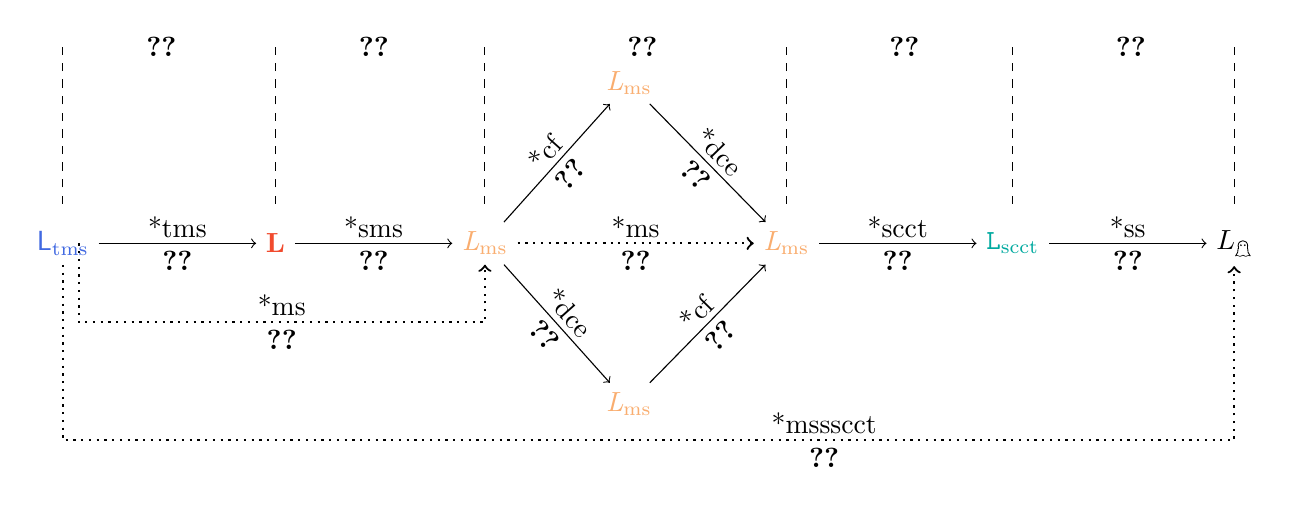
\begin{tikzpicture}
    \node (S) {$\src{L_{\tmssafe}}$};
    \node[right=2.0 of S] (T) {$\trg{L}$};
    \node[right=2.0 of T] (M) {$\irl{L_{\mssafe}}$};
    \node[below right=1.5 and 1.0 of M] (D0) {$\irl{L_{\mssafe}}$};
    \node[above right=1.5 and 1.0 of M] (C0) {$\irl{L_{\mssafe}}$};
    \node[right=3.0 of M] (E) {$\irl{L_{\mssafe}}$};
    \node[right=2.0 of E] (O) {$\obj{L_{\scctsafe}}$};
    \node[right=2.0 of O] (Z) {$\ird{L_{\mathghost}}$};

    \draw[->] (S) to[sloped] node[align=center] (tmsedge) {\gls*{tms}\\ \Cref{thm:cca:rtp:tms}} (T);
    \draw[->] (T) to[sloped] node[align=center] {\gls*{sms}\\ \Cref{thm:ccb:rtp:sms}} (M);
    \draw[->] (M) to[sloped] node[align=center] {\gls*{dce}\\ \Cref{thm:ccdce:rtp:ms}} (D0);
    \draw[->] (M) to[sloped] node[align=center] {\gls*{cf}\\ \Cref{thm:cccf:rtp:ms}} (C0);
    \draw[->] (D0) to[sloped] node[align=center] {\gls*{cf}\\ \Cref{thm:cccf:rtp:ms}} (E);
    \draw[->] (C0) to[sloped] node[align=center] {\gls*{dce}\\ \Cref{thm:ccdce:rtp:ms}} (E);
    \draw[->] (E) to[sloped] node[align=center] {\gls*{scct}\\ \Cref{thm:ccscct:rtp:scct}} (O);
    \draw[->] (O) to[sloped] node[align=center] {\gls*{ss}\\ \Cref{thm:ccspec:rtp:spec}} (Z);

    % Sections
    \node (sectms) at ($(S)+(1.25,2.5)$) {{\Cref{subsec:cs:tms}}};
    \node (secsms) at ($(T)+(1.25,2.5)$) {{\Cref{subsec:cs:ms}}};
    \node (secopts) at ($(M)+(2.0,2.5)$) {{\Cref{subsec:cs:opts}}};
    \node (secscct) at ($(E)+(1.5,2.5)$) {{\Cref{subsec:cs:scct}}};
    \node (secss) at ($(O)+(1.5,2.5)$) {{\Cref{subsec:cs:ss}}};

    \draw[thick,dotted,->] ($(S) + (0.2,0.0)$) to ($(S) - (-0.2,1)$) to node[align=center] {\gls*{ms}\\ \Cref{corr:ccab:rtp:ms}} ($(M) - (0.0,1)$) to (M);

    \draw[thick,dotted,->] (S) to ($(S) - (0.0,2.5)$) to node[align=center,pos=.65] {\gls*{mssscct}\\ \Cref{thm:ccall:rtp:mssscct}} ($(Z) - (0.0,2.5)$) to (Z);

    % \draw[thick,dotted,->] (S) to[bend right=33,sloped] node[align=center] {\gls*{ms}\\ \Cref{corr:ccab:rtp:ms}} (M);
    \draw[thick,dotted,->] (M) to[bend right=0,sloped] node[align=center] {\gls*{ms}\\ \Cref{thm:cccfccdce:rtp:ms}} (E);
%    \draw[thick,dotted,->] (S) to[out=-45,in=198,sloped] node[align=center] {\gls*{ms}+\gls*{scct}\\ \Cref{thm:ccall:rtp:msscct}} (O);
    % \draw[thick,dotted,->] (S) to[out=-40,in=210,sloped] node[align=center,pos=.8] {\gls*{mssscct}\\ \Cref{thm:ccall:rtp:mssscct}} (Z);

    \draw[dashed] ($(S)-(0.0,-0.5)$) -- ($(S)-(0.0,-2.5)$);
    \draw[dashed] ($(T)-(0.0,-0.5)$) -- ($(T)-(0.0,-2.5)$);
    \draw[dashed] ($(M)-(0.0,-0.5)$) -- ($(M)-(0.0,-2.5)$);
    \draw[dashed] ($(E)-(0.0,-0.5)$) -- ($(E)-(0.0,-2.5)$);
    \draw[dashed] ($(O)-(0.0,-0.5)$) -- ($(O)-(0.0,-2.5)$);
    \draw[dashed] ($(Z)-(0.0,-0.5)$) -- ($(Z)-(0.0,-2.5)$);
  \end{tikzpicture}
  \vspace{-1em}
  \caption{Visualisation of the optimising compilation pipeline that attains a combination of \gls*{ms} and \gls*{cct}. %
    Vertices in the graph are the programming languages from earlier sections (\Cref{sec:casestud:defs}). %
    All edges are secure compilers, but dotted edges use the presented framework (\Cref{sec:sequential}) and solid edges classic proof techniques. %
    The dashed lines partition the graph into the sections where the respective theorems are presented.
  }\label{fig:pipeline}
\end{figure*}
The section demonstrates the power of the framework (\Cref{sec:sequential}) by composing these compilers for a secure and optimising compilation chain that robustly preserves \gls*{mssscct}.
The first step in this chain is the compiler from $\src{L_{\tmssafe}}$ to $\trg{L}$ that robustly preserves just \gls*{tms} (\Cref{thm:cca:rtp:tms}).
From here, an instrumentation from $\trg{L}$ to $\irl{L_{\mssafe}}$ ensures that no out-of-bounds accesses can happen and, thus, programs at this point attain \gls*{sms} (\Cref{thm:ccb:rtp:sms}).
Since these properties compose into \gls*{ms}, composing these passes yields a compiler that robustly preserves \gls*{ms} (\Cref{corr:ccab:rtp:ms}).
Then, the section presents two optimising translations, namely \gls*{cf} and \gls*{dce}, each of which robustly preserves \gls*{ms} (\Cref{thm:ccdce:rtp:ms,thm:cccf:rtp:ms}).
These translations can be freely ordered in the compilation chain without compromising memory safety (\Cref{thm:cccfccdce:rtp:ms}).
The next step in the chain ensures that code stays \gls*{scct} (\Cref{thm:ccscct:rtp:scct}) when lowered from $\Lms$ to $\Lscct$, which is done by switching on a data-independent timing mode for the computation.
Lastly, by introducing barriers immediately after branches, speculative leaks via SPECTRE-PHT are prevented when compiling $\Lscct$ to $\Lspec$.
The final result is that the whole compilation chain robustly preserves \gls*{mssscct} (\Cref{thm:ccall:rtp:mssscct}).


\subsection{Robust Temporal Memory Safety Preservation}\label{subsec:cs:tms}

This subsection defines a secure compiler from $\Ltms$ to $\Ltrg$.
To this end, the compiler needs to ensure that when execution switches from context to component, the type signatures are respected.
It can do so by inserting dynamic typechecks prior to entering the body of a function belonging to the component:

\vspace{-1em}
{
\[
  \begin{array}{rcl}
    %\cca(\src{x}) = &\ \trg{x} 
    % \\
  	%&
  	%\qquad
    %\cca(\src{\lbinop{\expr[_{1}]}{\expr[_{2}]}}) = &\ \lbinop[\trg]{\left[\cca(\src{\expr[_{1}]})\right]}{\left[\cca(\src{\expr[_{2}]})\right]} \\
    %\cca(\src{n}) = &\ \trg{n} 
    % \\
    %&
    \cca(\src{\lget{x}{\expr}}) &= &\ \lget[\trg]{\trg{x}}{\left[\cca(\src{\expr})\right]} \\
    \cca(\src{\ldelete{x}}) &= &\ \ldelete[\trg]{\left[\cca(\src{x})\right]} \\
%    \cca(\src{\lset{x}{\expr[_{1}]}{\expr[_{2}]}}) & = \lset[\trg]{\left[\cca(\src{x})\right]}{\left[\cca(\src{\expr[_{1}]})\right]}{\left[\cca(\src{\expr_{2}})\right]} \\
\cca(\src{\lfunction{g}{x:\natt\to\type[_{e}]}{\expr}})  &= &\ \lfunction[\trg]{\trg{g}}{\trg{x}}{\lifz[\trg]{\trg{\lhast{x}{\natt}}}{
\\%
                                                         &  &
                                                            \left[\cca(\src{\expr})\right] %
                                                                                                 }{\labort[\trg]}}
  \end{array}
\]
}

The above sketches interesting parts, anything left out is a trivial ,,re-colouring'' from $\src{blue}$ to $\trg{red}$.

Since $\trg{L}$ has no static typing, a bogus context $\trg{\library_{\ctx}}$ can invoke a callable object accepting a $\src{\natt}$ with $\trg{\lpair{17}{29}}$.
By inserting a check, the compiler ensures that execution does not proceed in such cases.
%The compiler does not insert other checks and proceeds as the identity function (which in this paper amounts to a simple re-colouring of $\src{L_{\tmssafe}}$ to $\trg{L}$ expressions).

Compiling the \texttt{strncpy} function from \Cref{sec:introduction} with $\cca$, the compiler would in this case ensure that the arguments that are evaluated in the compiled \texttt{strncpy} are valid.
This effectively has no influence on the resulting trace, so a corresponding cross-language trace relation $\sim^{\Ltms}_{\Ltrg}$ is, up to one trace being $\src{blue}$ and the other $\trg{red}$, defined as equality.

$\cca$ is robustly preserving (\Cref{def:rtp}) \gls*{tms}:
\begin{theorem}[$\cca$ secure w.r.t. \gls*{tms}]\label{thm:cca:rtp:tms}
    $\rtp{\cca}{\tmssafe}$ % \Coqed
\end{theorem}

\subsection{Robust Spatial Memory Safety Preservation}\label{subsec:cs:ms}

This subsection defines spatial memory safety preserving compiler from $\Ltrg$ to $\Lms$, $\ccb$.
The compiler $\cc{\trg{L}}{\Lms}$ only inserts bounds-checks whenever reading from or writing to memory in order to enforce \gls*{sms}.
These bounds checks need the bounds information, which $\ccb$ keeps around by introducing a fresh identifier $\irl{x_{SIZE}}$ for each allocation that binds $\irl{x}$.
Then, it is simply a matter of referring to that variable and ensuring that memory accesses are in the interval $[\irl{0},\irl{x_{SIZE}})$.
For the case where it does not, the compiler inserts a panic.

\begin{nscenter}
% \small
  $$
  \begin{array}{rcl}
    \ccb(\trg{\lnew{x}{\expr[_{1}]}{\expr[_{2}]}}) & = 
                                                   & \llet[\irl]{\irl{x_{SIZE}}}{\ccb(\trg{\expr[_{1}]})}{}
    		\\&&
    		\lnew[\irl]{\irl{x}}{\irl{x_{SIZE}}}{\ccb(\trg{\expr[_{2}]})}
    		 \\
  \ccb(\trg{\lget{x}{\expr}}) & = 
                              & \llet[\irl]{\irl{x_{n}}}{\ccb(\trg{\expr})}{}
  	\\&&
  \lifz[\irl]{\irl{0\le x_{n}<x_{SIZE}}}{\\&&\irl{\lget{x}{x_{n}}}}{}
  		\irl{\labort}
  	  \\
  \ccb(\trg{\lset{x}{\expr[_{1}]}{\expr[_{2}]}}) & = 
                                                 & \llet[\irl]{\irl{x_{n}}}{\ccb(\trg{\expr[_{1}]})}{}
  		\\&&
  \lifz[\irl]{\irl{0\le x_{n}<x_{SIZE}}}{\\&&\lset[\irl]{\irl{x}}{\irl{x_{n}}}{}
  		\ccb(\trg{\expr[_{2}]})
  		}{\irl{\labort}} 
  		% \\
  \end{array}
  $$
\end{nscenter}

\begin{exampleenv}[Instrumented \texttt{strncpy}]
  Consider again \texttt{strncpy}, but instrumented for \gls*{sms}:
    \begin{lstlisting}[language=c,basicstyle=\ttfamily, morekeywords={size_t}]
void strncpy(size_t n, size_t dst_size, char *dst,
             size_t src_size, char *src) {
  for(size_t i = 0; i < src_size
      && src[i] != '\0' && i < n; ++i) {
    if(i < src_size && i < dst_size) {
      dst[i] = src[i];
    }
  }
}
    \end{lstlisting}
    Suppose context \texttt{strncpy(2, x, y)}, where \texttt{x} and \texttt{y} are pointers to valid regions of memory with allocated space for exactly two cells and do not contain the null-terminating character \texttt{'\textbackslash 0'}.
    When calling \texttt{strncpy} like this, the event $\ev{Use}\ \loc_{x}\ 2;\comp;\unlock$ would not be emitted during execution, since the bounds check prevents the condition \texttt{src[i] != '\textbackslash 0'} from executing.
\end{exampleenv}

Contrary to $\cca$, $\ccb$ may in fact change the trace of the original $\Ltrg$ program: if there is a memory access, it needs to be protected with a bounds check.
The corresponding relation $\sim^{\Ltrg}_{\Lms}$ that describes this semantic effect of the compiler may be sketched as follows:

{
\[
  \typerulenolabel{xrel:sms:read}{\trg{n}\text{ in bounds}}{\trg{Get\ \loc\ n;\comp}\sim^{\Ltrg}_{\Lms}\irl{Get\ \loc\ n;\comp}}
\]
\[
  \typerulenolabel{xrel:sms:panic}{\trg{n}\text{ out of bounds}}{\trg{Get\ \loc\ n;\comp}\sim^{\Ltrg}_{\Lms}\irl{\lightning}}
\]
}

And so on for the other, $\trg{Set}$ is analogous and any other event is just a trivial re-colouring.
Note that neither $\Ltrg$ nor $\Lms$ expose branches on the trace.
The bounds check is left abstract above, since the precise definition needs some technicalities that only inhibit readability without any technical insights.

It is possible to prove that $\ccb$ is robustly preserving \gls*{sms}.
\begin{theorem}[$\ccb$ secure w.r.t. \gls*{sms}]\label{thm:ccb:rtp:sms}
  $\rtpsim{\ccb}{\smssafe}{\sim^{\Ltrg}_{\Lms}}$ % \Coqed
\end{theorem}

Let $\src{\trace}\sim^{\Ltms}_{\Lms}\irl{\trace}:=\src{\trace}\sim^{\Ltms}_{\Ltrg}\bullet\sim^{\Ltrg}_{\Lms}\irl{\trace}$.

\Cref{corr:ccab:rtp:ms} states that the composition of $\cca$ and $\ccb$ is secure w.r.t. \gls*{ms} and follows from \Cref{thm:cca:rtp:tms,thm:ccb:rtp:sms} using \Cref{thm:rtpsim:sig}.

\begin{corollary}[$\cca\circ\ccb$ secure w.r.t. \gls*{ms}]\label{corr:ccab:rtp:ms}
  $\;$ 

  \begin{nscenter}
    $\rtpsim{\cca\circ\ccb}{\mssafe}{\sim^{\Ltms}_{\Lms}}$ % \Coqed
  \end{nscenter}
\end{corollary}

\Cref{thm:rtpsim:sig} has another precondition besides \Cref{thm:ccb:rtp:sms,thm:cca:rtp:tms}: $\sim^{\Ltms}_{\Ltrg}$ needs to be well-formed with respect to $\smssafe$.
This fact is easily established, since $\sim^{\Ltms}_{\Ltrg}$ is an equality. 

\begin{lemma}[$\sim^{\Ltms}_{\Ltrg}$ well-formed w.r.t. $\smssafe$]\label{lem:wf:ltmsltrg}
  $\wfcsig{\sim^{\Ltms}_{\Ltrg}}{\smssafe}$
\end{lemma}

\subsection{Optimising Compilers}\label{subsec:cs:opts} 

This section defines two optimising compiler passes from $\Lms$ to $\Lms$ which perform \gls*{dce} and \gls*{cf}, respectively.
The \gls*{dce} pass applies a naive rewrite rule on conditionals.
The \gls*{cf} pass relies on an auxiliary function \texttt{mix} that uses a substitutions accumulator $\irl{\substlist}$ in order to rewrite constant binary operations, e.g., $\irl{{17}-1}$ to $\irl{16}$, and replace variables that are assigned to constants, e.g., $\irl{\llet{x}{7}{x}}$ to $\irl{7}$.

\vspace{-1em}
\begin{gather*}
  \begin{align*}
    \ccdce(\irl{\lifz{true}{\expr[_{1}]}{\expr[_{2}]}}) & = \ccdce(\irl{\expr[_{1}]}) &\\
    \ccdce(\irl{\lifz{false}{\expr[_{1}]}{\expr[_{2}]}}) & = \ccdce(\irl{\expr[_{2}]}) &
  \end{align*}
  \\
  % \begin{align*}
  %   \ccdce(\irl{\lbinop{\expr[_{1}]}{\expr[_{2}]}}) & = \lbinop[\irl]{\ccdce(\irl{\expr[_{1}]})}{\ccdce(\irl{\expr[_{2}]})} &
  % \end{align*}
  % \\[0.25cm]
  \begin{align*}
    \cccf(\irl{\expr}) & = \partialeval{\irl{\expr}}{\irl{\hole{\cdot}}} &
  \end{align*}
  \\[0.125cm]
  \begin{align*}
   \partialeval{\irl{x}}{\irl{\substlist}} & = \irl{n} 
   	\qquad\qquad \text{if } \irl{\subst{n}{x}}\in\irl{\substlist} \\
   \partialeval{\irl{x}}{\irl{\substlist}} & = \irl{x} 
   \qquad\qquad \text{if } \irl{\subst{n}{x}}\notin\irl{\substlist} \\
   \partialeval{\irl{\lbinop{n}{m}}}{\irl{\substlist}} & = \irl{k} 
   \qquad\qquad \text{if } \lbinop{\irl{n}}{\irl{m}}=k \\
   %\partialeval{\irl{\lbinop{\expr[_{1}]}{\expr[_{2}]}}}{\irl{\substlist}} & = \lbinop[\irl]{\partialeval{\irl{\expr[_{1}]}}{\irl{\substlist}}}{\partialeval{\irl{\expr[_{2}]}}{\irl{\substlist}}} \\
   \partialeval{\irl{\llet{x}{\valueexpr}{\expr}}}{\irl{\substlist}} & = \partialeval{\irl{\expr}}{\irl{\subst{x}{\valueexpr}\cdot\substlist}} 
  % \\
  % \partialeval{\irl{\lget{x}{\expr}}}{\irl{\substlist}} & = \lget[\irl]{\irl{x}}{\partialeval{\irl{\expr}}{\irl{\substlist}}}
% \end{align*}
\end{align*}
% \\
% \begin{align*}
%   \partialeval{\irl{\llet{x}{\expr[_{1}]}{\expr[_{2}]}}}{\irl{\substlist}} & = \llet[\irl]{\irl{x}}{\partialeval{\irl{\expr[_{1}]}}{\irl{\substlist}}}{\\&\partialeval{\irl{\expr[_{2}]}}{\irl{\substlist}}} \\
%   \partialeval{\irl{\lifz{\expr[_{1}]}{\expr[_{2}]}{\expr[_{3}]}}}{\irl{\substlist}} & = \lifz[\irl]{\partialeval{\irl{\expr[_{1}]}}{\irl{\substlist}}}{\\&\partialeval{\irl{\expr[_{2}]}}{\irl{\substlist}}}{\partialeval{\irl{\expr[_{3}]}}{\irl{\substlist}}} \\
% \end{align*}
\end{gather*}
% \vspace{-3em}

Note that both passes have no effect on the resulting trace of a program, up to $\emptyevent$-steps. 
Because of this, both passes have equality as corresponding cross language trace relation. 
Moreover, it is straightforward to prove both passes as secure (\Cref{def:rtp}) w.r.t. \gls*{ms}. 

\begin{theorem}[$\ccdce$ secure w.r.t. \gls*{ms}]\label{thm:ccdce:rtp:ms}
  $\rtp{\ccdce}{\mssafe}$ %\Coqed
\end{theorem}
\begin{theorem}[$\cccf$ secure w.r.t. \gls*{ms}]\label{thm:cccf:rtp:ms}
  $\rtp{\cccf}{\mssafe}$ %\Coqe
\end{theorem}

With both \Cref{thm:ccdce:rtp:ms,thm:cccf:rtp:ms} it follows from \Cref{corr:swappable} that the two passes can be interchanged arbitrarily:

\begin{theorem}[$\cccf\circ\ccdce$ and $\cccf\circ\ccdce$ are secure w.r.t. \gls*{ms}]\label{thm:cccfccdce:rtp:ms}
  $\rtp{\cccf\circ\ccdce}{\mssafe}$ and $\rtp{\ccdce\circ\cccf}{\mssafe}$. % \Coqed
\end{theorem}

\subsection{Robust Strict Cryptographic Constant Time Preservation}\label{subsec:cs:scct}

This section defines a compiler $\ccscct$ from $\Lms$ to $\Lscct$ that robustly preserves \gls*{scct}. 
Given the fact that $\Lscct$ provides a \gls*{cct}-mode that can be turned on or off, the compiler inserts wrapper code for function calls and function bodies to ensure that execution in the component always happen in \gls*{cct}-mode.

\vspace{-1em}
\[
\begin{array}{rcl}
  \ccscct(\irl{\lfunction{g}{x}{\expr}}) & = & \lfunction[\obj]{\obj{g}}{\obj{x}}{\obj{\lwrdoit{ON};}\ccscct(\irl{\expr})} \\
  \ccscct(\irl{\lcall{g}{\expr}}) & = & \lcall[\obj]{\obj{g}}{\ccscct(\irl{\expr})\obj{; \lwrdoit{ON}}} 
    % \\
    % \ccscct(\irl{\lbinop{\expr[_{1}]}{\expr[_{2}]}}) & = \lbinop[\obj]{\ccscct{\irl{\expr[_{1}]}}}{\ccscct{\irl{\expr[_{2}]}}} 
    % \\
\end{array}
\]
% \vspace{-2em}
%
The context can overwrite the flag and exit the mode, but upon invoking a function that is part of the component, the flag would be set again.
Because of this, the semantic effect of the compiler, i.e., the corresponding cross-language trace relation $\sim^{\Lms}_{\Lscct}$, only relates events without secrets\footnote{For context actions, it can be whatever.}:

\begin{center} 
  \typerulenolabel{xrel:scct:noleak}{}{\irl{\preevent;\comp}\sim^{\Lms}_{\Lscct}\obj{\preevent;\comp;\unlock}}
\end{center}

The compiler is secure w.r.t. \gls*{scct}: %, similarly proven as in \Cref{subsec:cs:tms}.

\begin{theorem}[$\ccscct$ secure w.r.t. \gls*{scct}]\label{thm:ccscct:rtp:scct}
  \small
  $\rtpsim{\ccscct}{\scctsafe}{\sim^{\Lms}_{\Lscct}}$ % \Coqed
\end{theorem}

\subsection{Robust Speculative Safety Preservation}\label{subsec:cs:ss}

This section defines the final compilation pass $\ccspec$, which ensures that $\Lscct$ programs, which are assumed to be \gls*{ss}, stay \gls*{ss} at $\Lspec$-level. 
To do so, $\ccspec$ inserts a speculation barrier after branches, which is sufficient to harden the program against speculative leaks, since SPECTRE-PHT~\cite{kocher2019spectre} is the only speculative leak modeled in the semantics of $\Lspec$.

\vspace{-1em}
\[
\begin{array}{cl}
  &\ccspec{(\obj{\lifz{\expr[_0]}{\expr[_1]}{\expr[_2]}})} = 
  \\
  &\qquad\qquad \lifz[\ird]{\ccspec{\left(\obj{\expr[_0]}\right)}}{\ird{\lbarrier;}\ccspec{\left(\obj{\expr[_1]}\right)} \\&\qquad\qquad}{ \ird{\lbarrier;}\ccspec{\left(\obj{\expr[_2]}\right)}} 
\end{array}
\]
% \vspace{-2em}
%

Clearly, the corresponding cross-language trace relation $\sim^{\Lscct}_{\Lspec}$ has only one non-trivial case: For branches, only relate them where speculation is blocked by a barrier:

\begin{center}
  \typerulenolabel{xrel:spec:if}{}{\obj{Branch\ n}\sim^{\Lscct}_{\Lspec}\ird{Branch\ n}\cdot\ird{Spec}\cdot\ird{Barrier}\cdot\ird{Rlb}}
\end{center}

In the above, because of space constraints, pretend that each base-event has an additional $\obj{\comp;\securitytag}$, $\ird{\comp;\securitytag}$ annotation, so that full events are related.

With this, $\ccspec$ is secure with respect to \gls*{ss}.
\begin{theorem}[$\ccspec$ secure w.r.t. \gls*{ss}]\label{thm:ccspec:rtp:spec}
  \small$\rtpsim{\ccspec}{\sssafe}{\sim^{\Lscct}_{\Lspec}}$ % \Coqed
\end{theorem}

\subsection{Robust Preservation of Intersection of Memory Safety, Strict Cryptographic Constant Time, and Speculative Safety}

Finally, this subsection combines all previous results into one compilation chain to get that it preserves full \gls*{mssscct}.
Let $\ccmssscct$ be the compiler that is the composition of $\cca$, $\ccb$, $\cccf$, $\ccdce$, $\ccscct$, and $\ccspec$. 
Let $\sim^{\Ltms}_{\Lspec}$ be the composition of $\sim^{\Ltms}_{\Lms}$, $\sim^{\Lms}_{\Lscct}$, and $\sim^{\Lscct}_{\Lspec}$.
Then, the following corollary holds.

\begin{corollary}[$\ccmssscct$ secure w.r.t. \gls*{mssscct}]\label{thm:ccall:rtp:mssscct}
  $\;$ 

  \begin{nscenter}
    $\rtpsim{\cc{\Ltms}{\Lspec}}{\mssafe\cap\scctsafe\cap\sssafe}{\sim^{\Ltms}_{\Lspec}}$ % \Coqed
  \end{nscenter}
\end{corollary}

As with \Cref{corr:ccab:rtp:ms}, it is important to ensure that the respective cross language trace relations are well-formed (\Cref{def:wfc:sig:tracerel}).
It is already known that $\sim^{\Ltms}_{\Lms}$ is well-formed with respect to $\mssafe$ (\Cref{lem:wf:ltmsltrg}).
Next in the chain is $\sim^{\Lms}_{\Lscct}$, which has to be well-formed w.r.t. $\scctsafe$.
This lemma holds, since a trace that was $\scctsafe$ is $\scctsafe$ even after applying $\sim^{\Lms}_{\Lscct}$: The relation enforces that $\Lscct$ traces related to $\Lms$ traces have no leaks of secrets whatsoever.

\begin{lemma}[$\sim^{\Lms}_{\Lscct}$ well-formed w.r.t. $\scctsafe$]\label{lem:wf:lsmslscct}
  $\wfcsig{\sim^{\Lms}_{\Lscct}}{\scctsafe}$
\end{lemma}

The last relation is $\sim^{\Lscct}_{\Lspec}$ which needs to be well-formed w.r.t. $\sssafe$.
Similarly to the previous relation, this holds, since $\sim^{\Lscct}_{\Lspec}$ only relates $\Lspec$ traces, which do not have speculative leaks, with $\Lscct$ traces.

\begin{lemma}[$\sim^{\Lscct}_{\Lspec}$ well-formed w.r.t. $\sssafe$]\label{lem:wf:lscctlspec}
  $\wfcsig{\sim^{\Lscct}_{\Lspec}}{\sssafe}$
\end{lemma}

\section{Formal Insights}\label{sec:formalities}

This section provides some additional formal insights into the case study. 
\Cref{subsec:formalities:props} demonstrates that the resulting projected security property using the universal image (\Cref{def:universal:img}) is faithful to the original property. 
\Cref{subsec:compatsecpasses} discusses a caveat with \Cref{thm:rtpsim:sig}, while \Cref{subsec:seccompproofs} gives some additional background on the secure compilation proofs that do not use the compositionality framework (\Cref{sec:sequential}).
Lastly, \Cref{subsec:formalities:maps} discusses a minor technicality related to the ,,coloring'' of the investigated properties.

\subsection{Security Properties}\label{subsec:formalities:props}

When modeling some thing using formal methods, the intent is to do so faithfully. 
That is why it is important to ensure that the properties considered in \Cref{sec:casestud:rtp} follow this ideal.
It is relatively straightforward to see that, e.g., $\mssafe$ models a basic memory safety property. 
But, what about $\sigma_{\sim^{\Ltms}_{\Lms}}\left(\mssafe\right)$?
It is not immediately obvious that the resulting property after projecting it from $\Lms$-level to $\Ltms$-level is similar in spirit to the original $\mssafe$ property (\Cref{def:trace:msdef}) and this is what needs to be discussed when using the presented framework.
Let us investigate the involved projections from the case study.

\paragraph{$\sigma_{\sim^{\Ltms}_{\Lms}}\left(\mssafe\cap\scctsafe\cap\sssafe\right)$}
Consider a trace $\irl{\trace}\in\mssafe$ and remember that $\sim^{\Ltms}_{\Lms}$ is the composition of $\sim^{\Ltms}_{\Ltrg}$ and $\sim^{\Ltrg}_{\Lms}$.
{\em All} traces $\trg{\trace}$ with $\trg{\trace}\sim^{\Ltrg}_{\Lms}\irl{\trace}$ are almost identical to $\irl{\trace}$. 
They differ in memory accesses and crashes, where $\irl{\lightning}$ can be related to a $\trg{\lightning}$ or a memory event, e.g., $\trg{Get\ \loc\ 2}$.
In both cases, the memory access cannot be out of bounds. 

Now, consider all $\src{\trace}$ with $\src{\trace}\sim^{\Ltms}_{\Ltrg}\trg{\trace}$, which is like equality\footnote{Both $\sim^{\Ltms}_{\Ltrg}$ and $\sim^{\Ltrg}_{\Lms}$ filter context actions.}.

Therefore, the resulting projected property should faithfully model $\mssafe$, which translates to both $\scctsafe$ and $\sssafe$, since these properties trivially hold for $\Ltms$, $\Ltrg$, and $\Lms$ traces.


\paragraph{$\sigma_{\sim^{\Lms}_{\Lscct}}\left(\mssafe\cap\scctsafe\cap\sssafe\right)$}
Consider a trace $\obj{\trace}\in\scctsafe$ and all $\irl{\trace}$ such that $\irl{\trace}\sim^{\Lms}_{\Lscct}\obj{\trace}$. 
In turn, $\obj{\trace}$ cannot contain any leaks of secret values, so it cannot violate $\scctsafe$.
Toggling data-independent timing mode has no impact on $\mssafe$ or $\sssafe$.

\paragraph{$\sigma_{\sim^{\Lscct}_{\Lspec}}\left(\mssafe\cap\scctsafe\cap\sssafe\right)$}

The argument here is analogous to the previous one, introducing $\ird{barrier}$ never violates $\sssafe$ and has no effect on $\mssafe$ or $\scctsafe$.

\subsection{Compatibility of Secure Compiler Passes}\label{subsec:compatsecpasses}

\Cref{thm:rtpsim:sig} is always applicable, up to well-formedness of $\sim_1$ w.r.t. $\trg{\class[_2]}$.
However, consider $\ccb$ and $\ccspec$.
Even though swapping these compilers in the compilation chain is syntactically impossible, let us pretend that it is possible by just extending $\ccb$ for the constructs present in $\Lscct$ that are not present in $\Ltrg$.
Clearly, as evidenced earlier (\Cref{subsec:formalities:props}), $\ccb\cdot\ccspec$ is an acceptable composition that yields an interesting class of security properties, i.e., $\sigma_{\sim_{\irl{ms}}\bullet\sim_{\ird{\mathghost}}}\left(\mssafe\cap\scctsafe\cap\sssafe\right)$. 
However, swapping them $\ccspec\cdot\ccb$ means that $\ccb$ inserts new branches into the code that are not necessarily protected by a speculative execution barrier! 
It is crucial to ensure that the resulting class is meaningful, much similar to ensuring that a definition models what the formal methods expert intends to model. 
For the $\ccspec\cdot\ccb$ case, the class is $\sigma_{\sim_{\ird{\mathghost}}\bullet\sim_{\irl{ms}}}\left(\mssafe\cap\scctsafe\cap\sssafe\right)$
Since $\ev{Use\ \loc\ n}\sim_{\irl{ms}}\ev{Branch n}\cdot\ev{Spec}\cdots$, where $\cdots$ does not contain a $\ird{\ev{Barrier}}$ event, the resulting class of properties is only a subset of the intended one.
Because of this, it is crucial to analyze the precise shape of the class of properties after mapping a target-level property to a source-level property\footnote{Dito for mapping a source-level property to a target-level property.}.

\subsection{Secure Compilation Proofs}\label{subsec:seccompproofs}

The composition theorems can only be used on compilers which have been proven secure in the sense that they robustly preserve a certain class of properties. 
Traditional proof techniques apply, the usual strategy is to establish a backwards simulation between source components and their compiled target counterpart. 
For the universally quantified target context, a technique known as backtranslation is well-established, which constructs a source-level context either by backtranslating the target-level context, amounting to a ,,decompilation'', or by constructing it using the target-level trace, so that the source-context emits parts of the whole execution trace that are related to the parts emitted by the target-level context. 
Up to backtranslations for $\ccdce$ and $\cccf$, all backtranslations in the case-study are trace based, while for $\ccdce$ and $\cccf$, they are context-based. 
Since these optimisations have no significant semantic effect and source- and target-language are equal, the backtranslation amounts to an identity translation. 

\subsection{Mapping Language-Specific to Property-Specific Traces}\label{subsec:formalities:maps}

Previous sections disregarded a glaring but minor technical issue: Take $\tmssafe$ (\Cref{def:trace:tmsdef}) as an example.
It contains traces as specified in \Cref{subsec:basic:memsafety:tracemodel}.
However, these are different from $\Ltms$ traces (\Cref{subsec:ltms}) which means that \Cref{thm:wt:tms} is ,,ill-typed''.
Similarly for the other theorems.
In the interest of reducing visual baggage, the notation left out yet another cross-language trace relation, translating language-specific traces into these non-language specific traces. 
In doing so, context-level actions are dropped and, e.g., both $\src{Get\ \loc\ n}$ and $\src{Set\ \loc\ n}$ are translated into $\ev{Use\ \loc\ n}$.

\section{Related Work\pages{2}}\label{sec:relwork}

This section discusses work on robust compilation (\Cref{subsec:relw:seccomprtp}) and on other secure compilation criteria (\Cref{subsec:relw:seccompcrit}).
Since the case study of \Cref{sec:casestud:defs,sec:casestud:rtp} implements measures for preserving \gls*{ms}, \gls*{cct}, and \gls*{ss}, this section then presents relevant related work as well (\Cref{subsec:relw:msmechs,subsec:relw:cctmechs,subsec:relw:ssmechs}).

\subsection{Secure Compilation as Robust Preservation}\label{subsec:relw:seccomprtp}

The robust preservation of properties as a compiler-level criterion has been analyzed extensively~\cite{abate2019jour,patrignani2021rsc,abate2021extacc,patrignani2019survey} and thus we build on that framework.
No existing work is concerned with composing robustly safe compilers.
%Parts of these works consider languages with different trace models and our technical setup can handle this. 
The work relating robust preservation with universal composability~\cite{patrignani2022universal} is closest to what this paper presents.
The authors demonstrate a similar compositionality theorem to what is presented here (\Cref{sec:sequential}) but use it in the context of protocols.
The work is missing the upper and lower compositions as well as the generality to support different trace models.
% The authors demonstrate a similar compositionality theorem to what is presented here (\Cref{sec:sequential}) as well as in an earlier version of this work~\cite{kruse2022csc}.
% However, they do not demonstrate the scalability of the approach by means of a case study.

\subsection{Other Secure Compilation Criteria}\label{subsec:relw:seccompcrit}

While this paper focuses on the robust preservation framework~\cite{abate2019jour}, other secure compilation criteria exist.
The survey on formal approaches to secure compilation~\cite{patrignani2019survey} discusses a broad spectrum already, while this section presents a very high-level overview.
Fully abstract compilation~\cite{abadi1999fullabstraction} states that a compiler should preserve and reflect observational equivalence between source and target programs.
It was shown~\cite{abate2021faandrc} that fully abstract compilers robustly preserve program properties that are either trivial or meaningless.
As a mitigation for this, the authors presented a categorical approach based on maps of distributive laws~\cite{watanabe2002modl}, which they call many maps of distributive laws.
Maps of distributive laws have been investigated before as a possible secure compilation criterion~\cite{tsampas2020catsc}.
Other approaches are extensions of the compiler correctness criterion as discussed in other work~\cite{patterson2019next700} or the introduction of opaque observations~\cite{vu2021reconciling} to reconcile compiler optimisations with security.
Note that this work also presents secure compilers that are optimising, but contrary to the other~\cite{vu2021reconciling}, provides a formal account of these in the robust preservation framework.
% Lastly, the authors of this paper have presented ongoing work~\cite{patrignani2023blame} on a weaker robust preservation criteria based on the concept blame.

\subsection{Memory Safety Mechanisms}\label{subsec:relw:msmechs}

Different mechanisms for enforcing memory safety exist that also consider the secure compilation domain, i.e., have an active attacker model.
For example, the ,,pointers as capabilities'' principle represents pointers as machine-level capabilities~\cite{korashy2021capableptrs}, which behave in a similar fashion to capabilities by means of linear typing~\cite{morrisett2005L3}.
The approach of this paper also uses linear typing, but differs from $L^{3}$~\cite{morrisett2005L3} in the way that functions are not first-class.
Moreover, this paper considers an active attacker, while the work on $L^{3}$ only discusses whole programs and, thus, has no active attacker model.
The instrumentation to ensure memory safety that this paper presents is inspired by Softbounds~\cite{nagarakatte2009soft}.
That work inserts bounds-checks in front of pointer-dereferences and, for this to work, inserts meta-data information on pointer creation.
Softbounds also works in a more advanced setting with structured fields accesses and also introduces a table-lookup for pointers that are stored in memory.
This paper only considers arrays of primitive data, i.e., there are no pointers to pointers or structures.
Several other approaches to memory-safety exist in literature, specifically as compiler instrumentations~\cite{akritidis2009baggy,younan2010paricheck,jung2021pico,shankaranarayana2023tailcheck,dhumbumroong2020boundwarden,nam2019framer,zhou2023fatptrs}, hardware-extensions~\cite{kwon2013lowfat,saileshwar2022heapcheck,chen2023flexpointer,kim2023whistle}, or programming language extensions~\cite{elliott2018checkedc,li2022formalcheckedc,jim2002cyclone,elliott2015guilt,west2005cuckoo,weis2019fyr,benoit2019uniqueness}.
What differentiates this work from them is that this work uses known, compiler-based approaches to ensure memory-safety as a means to investigate secure compiler compositions.
This paper does not provide efficient memory-safety, but serves as a theoretical foundation for the secure compilation domain.

To extend the languages in this paper with a less restricted form of pointer arithmetic, the region coloring memory safety monitor presented in earlier work~\cite{michael2023mswasm} can be used.
The work presenting this monitor provides an approach for the robust preservation of memory safety compiling from C to WASM.
However, they do not discuss composition of secure compilers but rather investigate an instance of a secure compiler.

\subsection{Cryptographic Constant Time Mechanisms}\label{subsec:relw:cctmechs}

The approach to preserving cryptographic constant time in this paper is high-level, where a programming language exposes a way to switch the semantics to a data (operand) independent timing mode.
Since identifiers in $\Lscct$ are annotated with a secrecy tag, this approach is similar to others with information flow control.
For example, Vale~\cite{bond2017vale} uses Dafny to ensure constant-time assembly code, while Jasmin~\cite{almeida2017jasmin} makes use of the Coq proof assistant to reject non-constant-time programs.
CT-Wasm~\cite{watt2019ctwasm} enforces constant-timeness by means of a type system.
Different to the approach of this paper, these approaches necessitate that the programmer writes \gls*{cct} code.
An approach to allow programmers to write more high-level code is CryptOpt~\cite{kuepper2023cryptopt}, which generates efficient target-code by means of a randomised search.
This paper abstracts over concrete mitigation strategies and simply assumes that there is a flag to switch to a cryptographic-constant time execution mode.
This can be realised by employing the FaCT~\cite{cauligi2019fact} compiler, which translates common non-constant time code patterns to be constant-time, and the data (object) independent timing execution mode of modern processors.

\subsection{Speculation Safety Mechanisms}\label{subsec:relw:ssmechs}

With the advent of speculative execution in processors, it is possible to exploit this unusual paradigm identify secrets.
SPECTECTOR~\cite{guarnieri2018spectector} models speculative execution formally and the present work has taken inspiration in the sematics of $\Lspec$ and in \Cref{def:trace:ss} from SPECTECTOR.
A subsequent line of work~\cite{fabian2022automatic} shows how to modularly define and compose formal semantics that models different speculative execution variants. 
Similar in spirit, recent work~\cite{fabian2024lift} demonstrates how to lift existing secure compilation proofs for security properties related to speculative execution to more powerful properties, i.e., properties defined for languages with a trace model that enables more vulnerabilities, such as combinations of different speculative execution exploits. 
To this end, they define a lifting framework and demonstrate how a secure compilation proof for a weaker property can be lifted to a stronger one. 
Contrary to the compositionality framework presented in this paper, these works are only concerned with composing semantics of the respective programming languages, while in this paper, the secure compilers themselves are composed.

\section{Conclusion\pages{$\sfrac{1}{2}$}}\label{sec:concl}
This paper tackles the problem of understanding what kind of security properties a secure compiler preserves, when said compiler is the combination of compiler passes that preserve possibly different security properties.
% 
%For this, this paper first formalised security properties of interest and their composition.
% 
The paper proves that composing secure compilers that preserve certain properties results in a secure compiler that preserves the composition of these properties.
% While the presented security property composition relied on monitors that check only trace-properties, the composition of secure compilers does not make any restriction towards the kind of property involved in the composition. 
% It is subject to future work to develop techniques to verify relational hyperproperties~\cite{abate2019jour}, while the composition of hyperproperties could be very similar to the composition of ordinary properties as presented in this paper, since hyperproperties can be checked with an automata-based model-checker~\cite{beutner23hyperltl}.
% 
Finally, this paper defines a multi-pass compiler and proves that it preserves \gls*{mssscct}.
Crucially, this paper derives the security of the multi-pass compiler from the composition of the security properties preserved by its individual passes, which include security-preserving as well as optimisation passes.
% For future work, it is interesting to look at more sophisticated optimisation passes that, e.g., reorder events that appear on traces.


% \newpage

\bibliographystyle{IEEEtran}
\bibliography{main}

%%
%% If your work has an appendix, this is the place to put it.
% \appendix

\end{document}
\endinput
